\newcommand{\econtexRoot}{Paper/}
% The \commands below are required to allow sharing of the same base code via Github between TeXLive on a local machine and ShareLaTeX.  This is an ugly solution to the requirement that custom LaTeX packages be accessible, and that ShareLaTeX seems to ignore symbolic links (even if they are relative links to valid locations)
\providecommand{\econtex}{\econtexRoot/texmf-local/tex/latex/econtex}
\providecommand{\econtexSetup}{\econtexRoot/texmf-local/tex/latex/econtexSetup}
\providecommand{\econtexShortcuts}{\econtexRoot/texmf-local/tex/latex/econtexShortcuts}
\providecommand{\econtexBibMake}{\econtexRoot/texmf-local/tex/latex/econtexBibMake}
\providecommand{\econtexBibStyle}{\econtexRoot/texmf-local/bibtex/bst/econtex}
\providecommand{\notes}{\econtexRoot/texmf-local/tex/latex/handout}
\providecommand{\handoutSetup}{\econtexRoot/texmf-local/tex/latex/handoutSetup}
\providecommand{\handoutShortcuts}{\econtexRoot/texmf-local/tex/latex/handoutShortcuts}
\providecommand{\handoutBibMake}{\econtexRoot/texmf-local/tex/latex/handoutBibMake}
\providecommand{\handoutBibStyle}{\econtexRoot/texmf-local/bibtex/bst/handout}

  

\documentclass{beamer}
\usepackage{remreset}
\usepackage{etoolbox}
\usepackage{comment}
\usepackage{graphicx}
%\usepackage{dtklogos}
\usepackage{dsfont}
\usepackage{amsmath,amssymb}
\usepackage{\econtexShortcuts}
\usepackage[english]{babel}
\usepackage{tikz} 
\usetikzlibrary{tikzmark,fit,shapes.geometric}
\usetikzlibrary{tikzmark,calc,arrows,shapes,decorations.pathreplacing}
\tikzset{every picture/.style={remember picture}}
\usepackage{cancel}
\usepackage{booktabs,natbib}
\setbeamercovered{invisible}

\usepackage{dcolumn}


\makeatletter
\@removefromreset{subsection}{section}
\patchcmd{\beamer@part}{\setcounter{subsection}{0}}{}{}
\makeatother
\setcounter{subsection}{1}
\setbeamercovered{transparent}
\setbeamertemplate{navigation symbols}{}%remove navigation symbols
\begin{comment}
\setbeamertemplate{footline}
{
	\hbox{\begin{beamercolorbox}[wd=1\paperwidth,ht=2.25ex,dp=1ex,right]{framenumber}%
			\usebeamerfont{framenumber}\insertframenumber{} \hspace*{2ex}
	\end{beamercolorbox}}%
	\vskip0pt%
}
\end{comment}


\mode<presentation>{}
%% preamble
\title[Consumption Heterogeneity: Micro Drivers and Macro Implications]{Consumption Heterogeneity: \\ Micro Drivers and Macro Implications}
\author{Edmund Crawley \& Andreas Kuchler}
\date[17/10/2019]{Alternative datasets for macro analysis and monetary policy\\Banque de France / Bocconi University\\ October 17, 2019}
\usetheme{Frankfurt}

\setbeamertemplate{navigation symbols}{}
\makeatletter
\setbeamertemplate{footline}
{%
	\hbox{\begin{beamercolorbox}[wd=1\paperwidth,ht=2.25ex,dp=1ex,right]{framenumber}%
		\usebeamerfont{framenumber}\insertframenumber{} \hspace*{2ex}
	\end{beamercolorbox}}%
	\vskip0pt%
	\pgfuseshading{beamer@barshade}%
	\ifbeamer@sb@subsection%
	\vskip-9.75ex%
	\else%
	\vskip-7ex%
	\fi%
	\begin{beamercolorbox}[ignorebg,ht=2.25ex,dp=3.75ex]{section in head/foot}
		\insertnavigation{\paperwidth}
	\end{beamercolorbox}%
	\ifbeamer@sb@subsection%
	\begin{beamercolorbox}[ignorebg,ht=2.125ex,dp=1.125ex,%
		leftskip=.3cm,rightskip=.3cm plus1fil]{subsection in head/foot}
		\usebeamerfont{subsection in head/foot}\insertsubsectionhead \insertframenumber{} \hspace*{2ex}
	\end{beamercolorbox}%
	\fi%
}%
\setbeamertemplate{headline}{%
}
\makeatother
\begin{document}
\newcolumntype{d}[1]{D{.}{.}{#1}}
%circled draws a circle around a number
\newcommand*\circled[1]{\tikz[baseline=(char.base)]{
		\node[shape=circle,draw,inner sep=2pt] (char) {#1};}}

\begin{frame}[plain]
\titlepage
\end{frame}
\addtocounter{framenumber}{-1}
\section{Introduction}
\setbeamercovered{invisible}
\frame
{
	\frametitle{What Do We Do?}
	\begin{center}
	We estimate the \textbf{sensitivity of consumption} \\
	\bigskip
	 to permanent and transitory \textbf{shocks to income} \\
	 \bigskip
	 for \textbf{different groups} of households
	 \end{center}
}
\frame[t]
{
	\frametitle{Hasn't This Been Done Before?}
	\vspace{1.8cm}
	Yes, but...\\
	\bigskip
	\hspace{1cm} Our \textbf{method} addresses bias in previous results  \tikz[baseline]{\node(bias){}}\\
	\bigskip
	\hspace{1cm} Our \textbf{data} allows sharp focus on household heterogeneity  \tikz[baseline]{\node(data){}}\\ 
	\only<2->{
	\begin{tikzpicture}[remember picture,overlay]
	\node (bias1a)  at ([shift={(-3.5,0.3)}]bias) {};
	\node (bias1b)  at ([shift={(0,1)}]bias1a) {};
	\draw[blue,thick,->] (bias1a)  to [in=270,out=90] (bias1b) node[anchor=south,text = blue] {Time Aggregation Problem};
	\end{tikzpicture}
	}
	\only<2->{
	\begin{tikzpicture}[remember picture,overlay]
	\node (data1a)  at ([shift={(-8.2,-0.0)}]data) {};
	\node (data1b)  at ([shift={(0.5,-1)}]data1a) {};
	\draw[blue,thick,->] (data1a)  to [in=180,out=270] (data1b) node[anchor=west,text = blue] {\begin{tabular}{l} Sample size in millions\\ Detailed balance sheet \end{tabular}};
	\end{tikzpicture}
	}
}
\frame
{
	\frametitle{Why Do We Care? (as macroeconomists)}
	1) Heterogenous agent models have testable micro behavior \tikz[baseline]{\node(micro){}}\\
	\bigskip
	2) Quantify Macro Implications \tikz[baseline]{\node(macro){}}
	\only<2->{
	\begin{tikzpicture}[remember picture,overlay]
	\node (micro1a)  at ([shift={(-2.2,0.3)}]micro) {};
	\node (micro1b)  at ([shift={(-1,0.8)}]micro1a) {};
	\draw[blue,thick,->] (micro1a)  to [in=270,out=90] (micro1b) node[anchor=south,text = blue] {\begin{tabular}{l} e.g. Consumption smoothing requires liquid wealth  \end{tabular}};
	\end{tikzpicture}
	\begin{tikzpicture}[remember picture,overlay]
	\node (macro1a)  at ([shift={(-2.8,0.0)}]macro) {};
	\node (macro1b)  at ([shift={(-0.0,-0.8)}]macro1a) {};
	\draw[blue,thick,->] (macro1a)  to [in=90,out=270] (macro1b) node[anchor=north,text = blue] {\begin{tabular}{l} e.g. Redistribution in Monetary Policy  \end{tabular}};
	\end{tikzpicture}
	}
}
\frame[t]
{
	\frametitle{What do we find? (Redistribution in Monetary Policy)}
	\only<1>{
		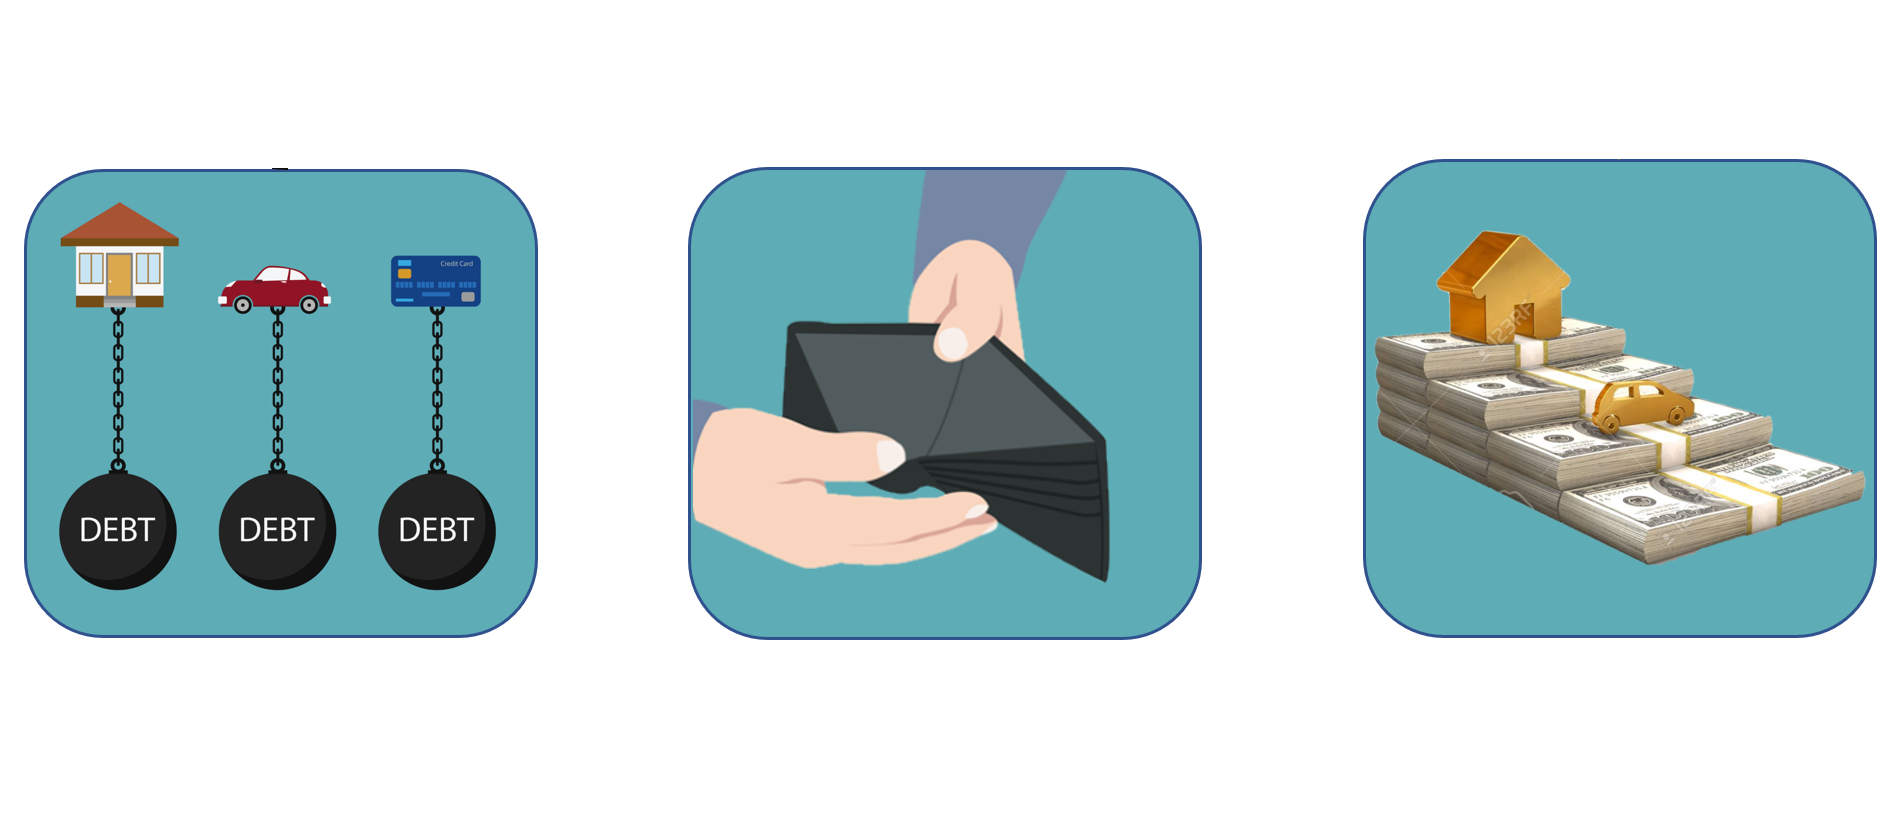
\includegraphics[width=11cm]{./SlideFigures/IRE_Big1.png}
	}
	\only<2>{
	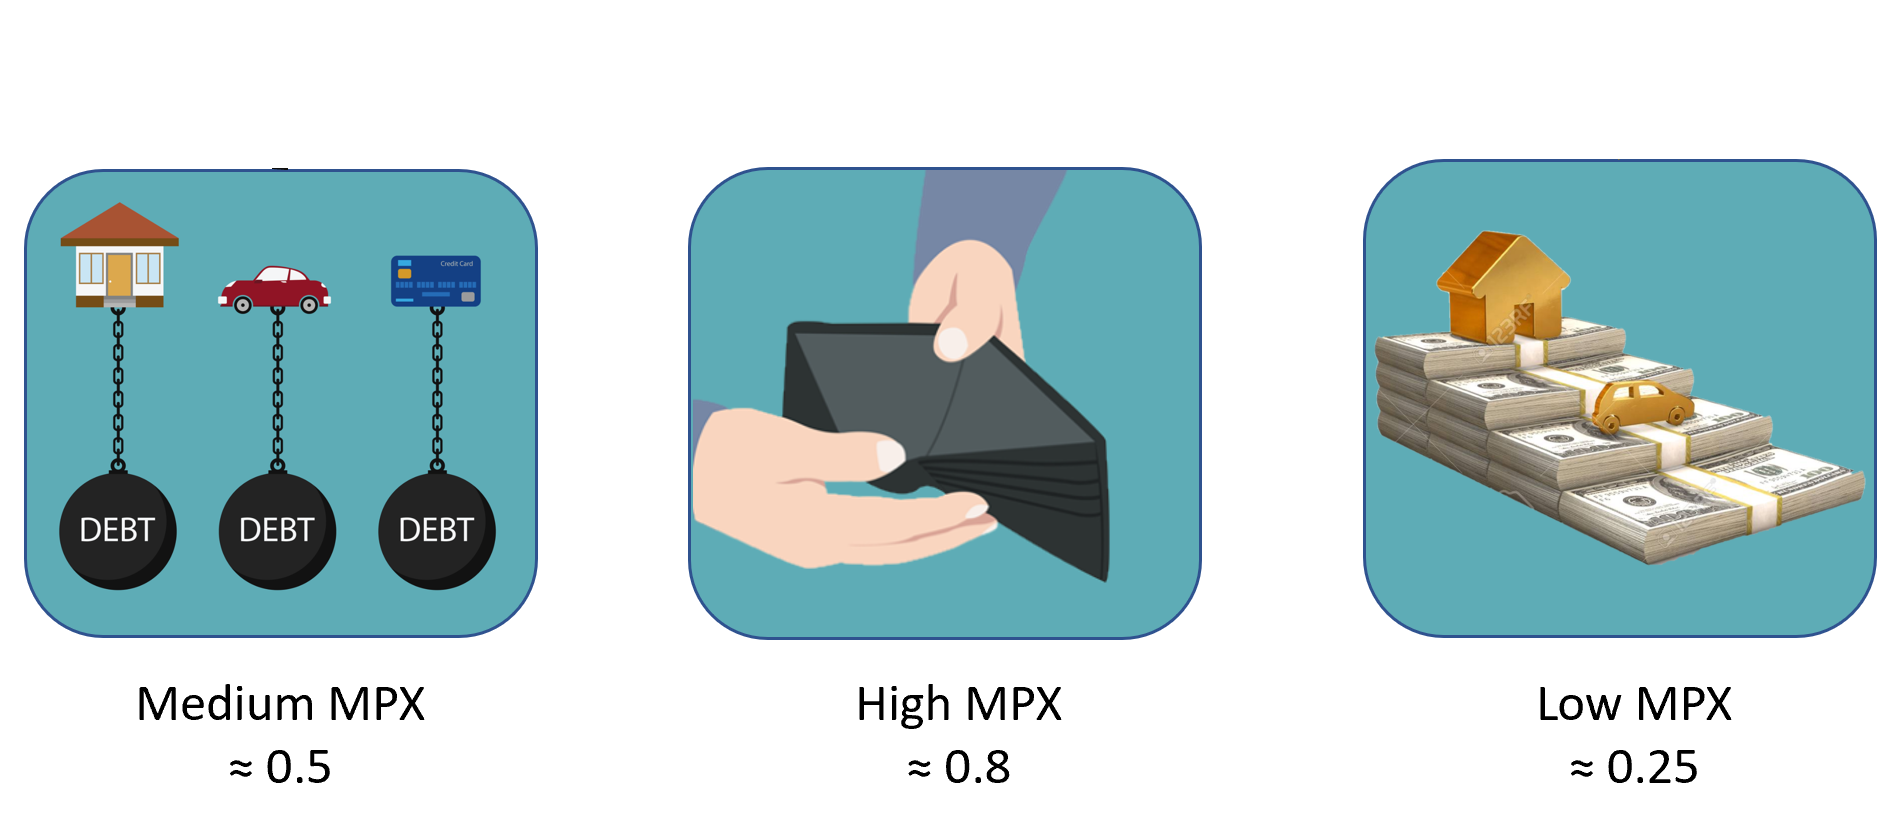
\includegraphics[width=11cm]{./SlideFigures/IRE_Big2.png}
	\\[0.7cm]
	MPX: Marginal Propensity to eXpend (includes durables)
	}
	\only<3->{
	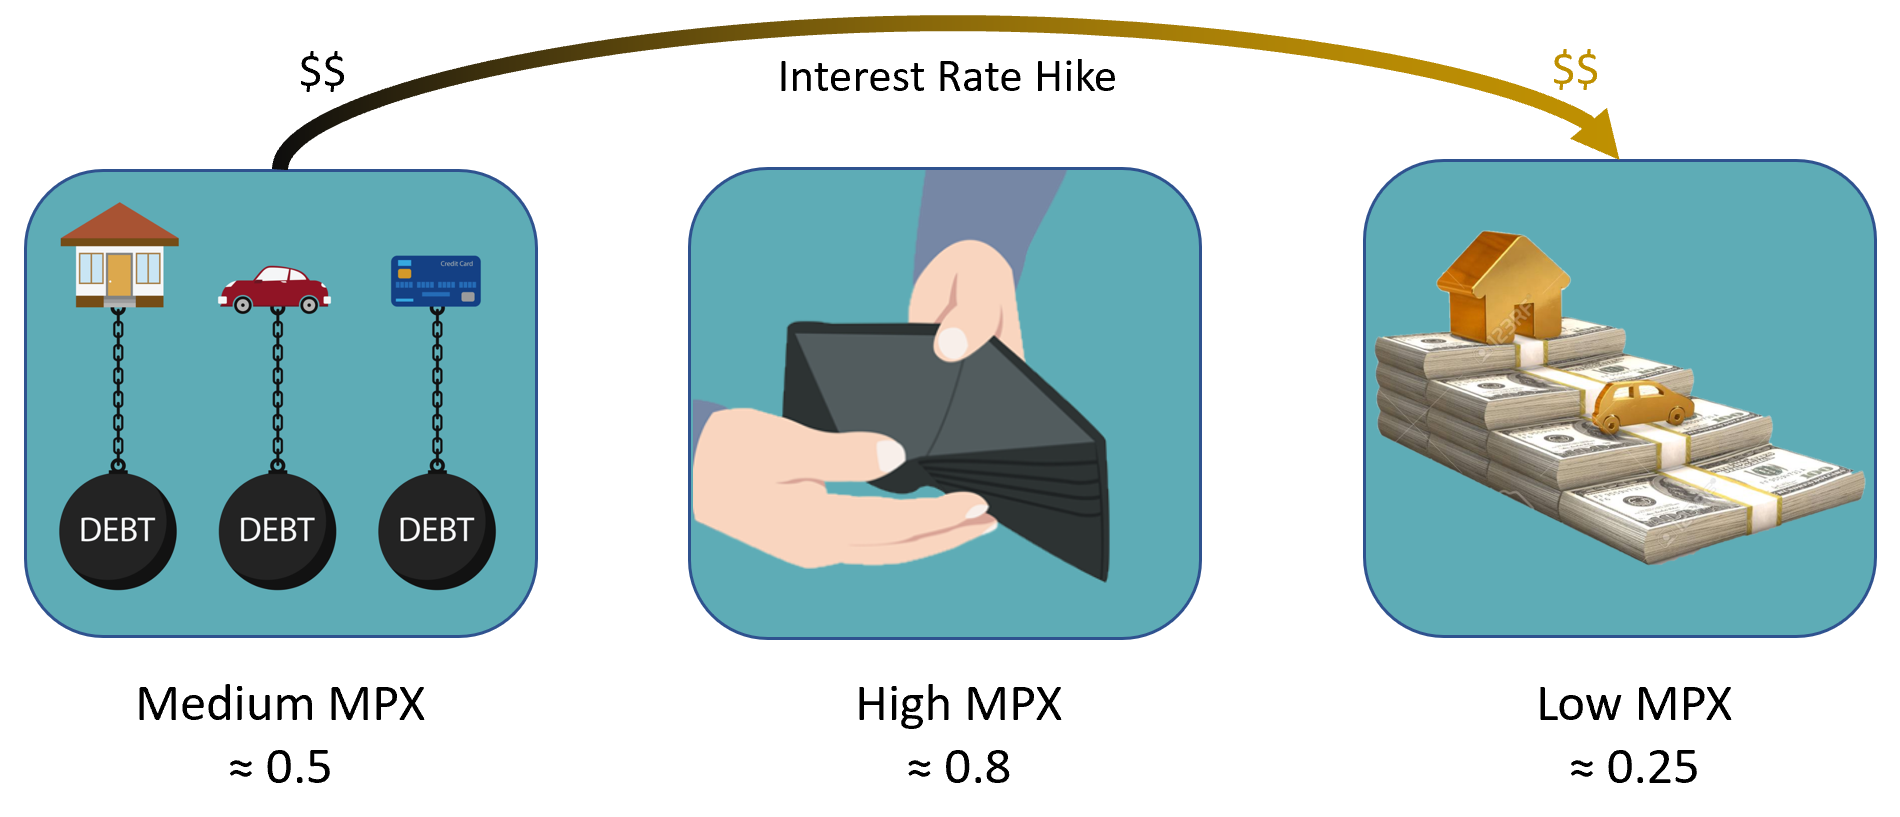
\includegraphics[width=11cm]{./SlideFigures/IRE_Big3.png} \tikz[baseline]{\node(ire){}}
	}
	\only<3>{
	\begin{tikzpicture}[remember picture,overlay]
	\node (ire1a)  at ([shift={(-9.5,0.1)}]ire) {};
	\node (ire1b)  at ([shift={(-0.4,-0.4)}]ire1a) {};
	\draw[blue,thick,->] (ire1a)  to [in=45,out=225] (ire1b) node[anchor=north,text = blue] {\begin{tabular}{l} Decrease spending \\ a \textit{lot}  \end{tabular}};
	\node (ire1c)  at ([shift={(-1.5,0.1)}]ire) {};
	\node (ire1d)  at ([shift={(0.4,-0.4)}]ire1c) {};
	\draw[blue,thick,->] (ire1c)  to [in=135,out=315] (ire1d) node[anchor=north,text = blue] {\begin{tabular}{r} Increase spending \\ a \textit{little}  \end{tabular}};
	\end{tikzpicture}
	}
	\only<4->{
	\vspace{-.5cm}
	\begin{align*}
	\text{1yr rate }&\uparrow \ 1\% \\
	\tikz[baseline]{\node(aggregate){}} \textit{Aggregate}\text{ Spending }&\downarrow \ 26 \text{ basis points}
	\end{align*}
	\begin{tikzpicture}[remember picture,overlay]
	\node (aggregatea)  at ([shift={(1.5,-0.1)}]aggregate) {};
	\node (aggregateb)  at ([shift={(-0.4,-0.4)}]aggregatea) {};
	\draw[blue,thick,->] (aggregatea)  to [in=45,out=225] (aggregateb) node[anchor=north,text = blue] {Through this redistribution channel \textit{alone}};
	\end{tikzpicture}
	}
}
\section{Empirical Strategy}
\setbeamercovered{invisible}
\frame[t]{
	\frametitle{Reduced Form Approach}
	Identifying Restrictions on\\
	\bigskip
	\hspace{1cm}\textbf{Income}\tikz[baseline]{\node(income){}}\\
	\bigskip
	\hspace{1cm}and\\
	\bigskip
	\hspace{1cm}\textbf{Consumption}\tikz[baseline]{\node(consumption){}}\\
	\bigskip
	In \textbf{Continuous} Time\tikz[baseline]{\node(continuous){}}\\
	\vspace{0.8cm}
	\only<2->{
	\begin{tikzpicture}[remember picture,overlay]
	\node (incomea)  at ([shift={(0,0.1)}]income) {};
	\node (incomeb)  at ([shift={(2,0)}]incomea) {};
	\node (consumptiona)  at ([shift={(0,0.1)}]consumption) {};
	\node (consumptionb)  at ([shift={(1,0)}]consumptiona) {};
	\draw[blue,thick,->] (incomea)  to [in=180,out=0] (incomeb) node[anchor=west,text = blue] {\begin{tabular}{lcl}  Permanent & (random walk) & shocks\\ Transitory & ($<$2 years) & shocks  \end{tabular}};
		\end{tikzpicture}
	}
	\only<3->{
	\begin{tikzpicture}[remember picture,overlay]
	\draw[blue,thick,->] (consumptiona)  to [in=180,out=0] (consumptionb) node[anchor=west,text = blue] {\begin{tabular}{lcl} Permanent & (random walk) & response\\ Transitory & ($<$2 years) & response  \end{tabular}};
	\end{tikzpicture}
	}
	\only<4->{
	\begin{tikzpicture}[remember picture,overlay]
	\node (continuousa)  at ([shift={(0,0.1)}]continuous) {};
	\node (continuousb)  at ([shift={(1,0)}]continuousa) {};
	\draw[blue,thick,->] (continuousa)  to [in=180,out=0] (continuousb) node[anchor=west,text = blue] {\begin{tabular}{lcl} Time Aggregation Problem  \end{tabular}};
	\end{tikzpicture}
	}
%	\only<5->{
%	\centering
%	\hspace{-1.17cm}But first some intuition: Na\"ively Regress \\
%	\bigskip
%	 Change in Consumption on Change in Income (over N years)
%	}
}
%\frame[t]
%{
%	\frametitle{Na\"ive Regression: Consumption Growth on Income Growth}
%	\vspace{-0.5cm}
%	\begin{align*}
%	\Delta^N c_i = \alpha^N + \beta^N \Delta^N y_i +\varepsilon_i
%	\end{align*}
%	\centering
%	\begin{tikzpicture}
%	\node (img1) {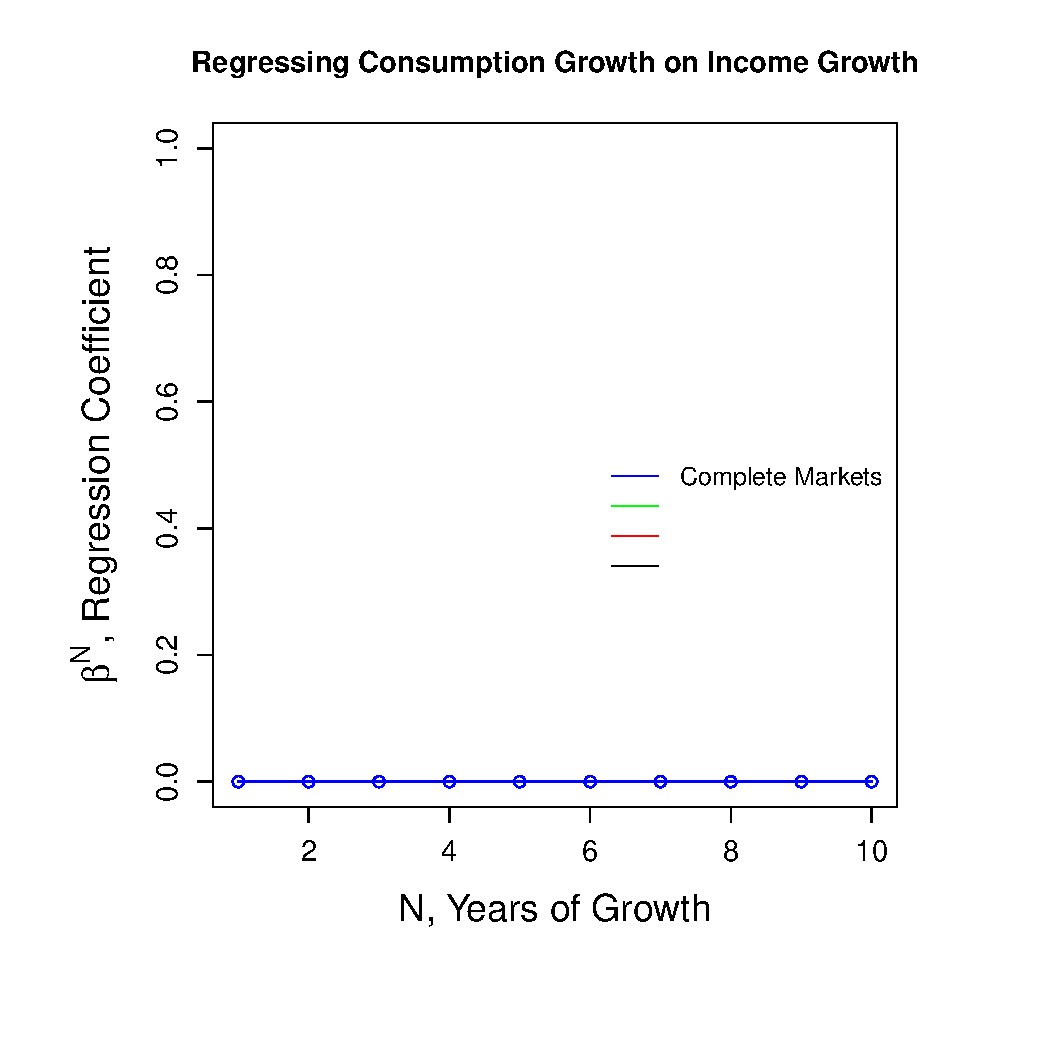
\includegraphics[height=7.5cm,trim= 0 0 0 2cm,clip]{../Figures/basic_regression_complete_level_lincome_head.pdf}};
%	\pause
%	\node (img2) {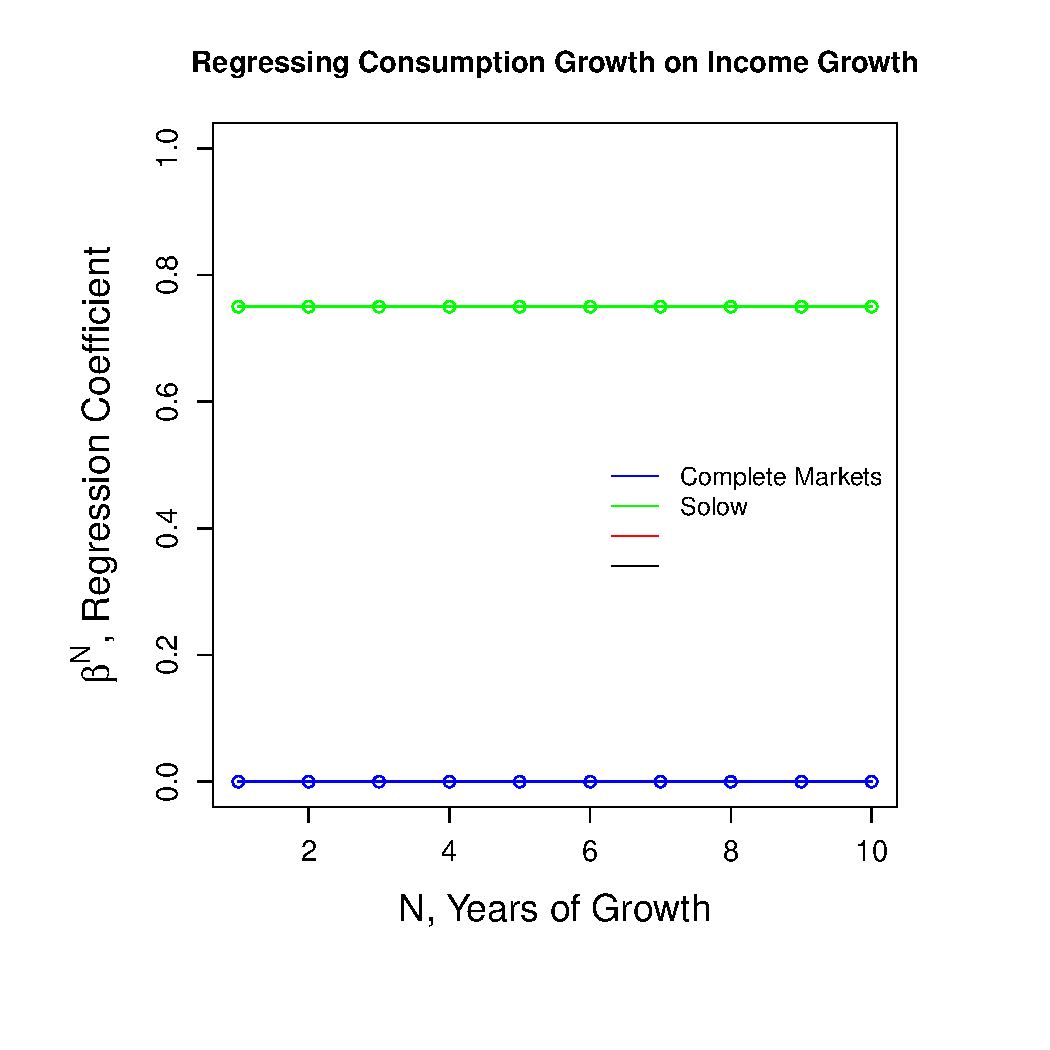
\includegraphics[height=7.5cm,trim= 0 0 0 2cm,clip]{../Figures/basic_regression_solow_level_lincome_head.pdf}};
%	\pause
%	\node (img3) {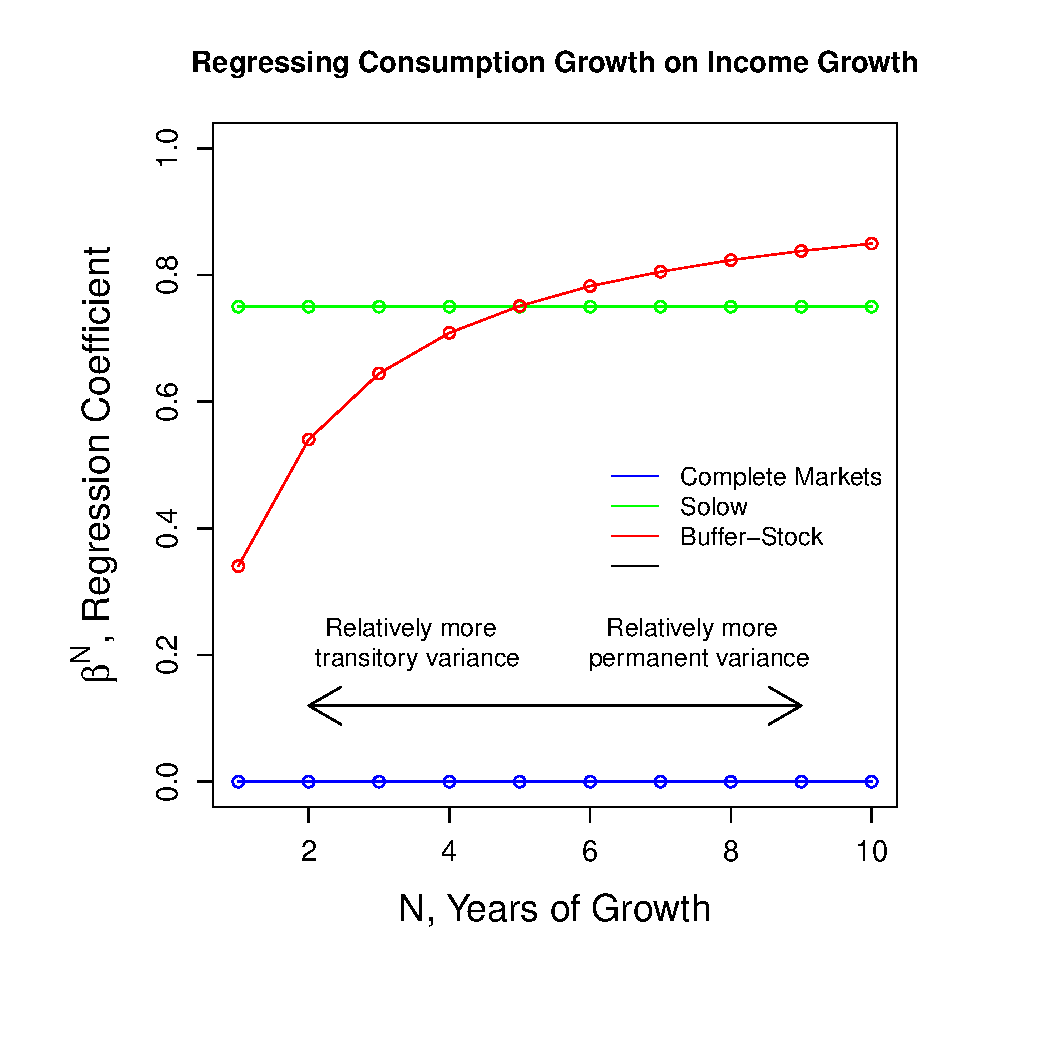
\includegraphics[height=7.5cm,trim= 0 0 0 2cm,clip]{../Figures/basic_regression_BS_level_lincome_head.pdf}};
%	\pause
%	\node (img4) {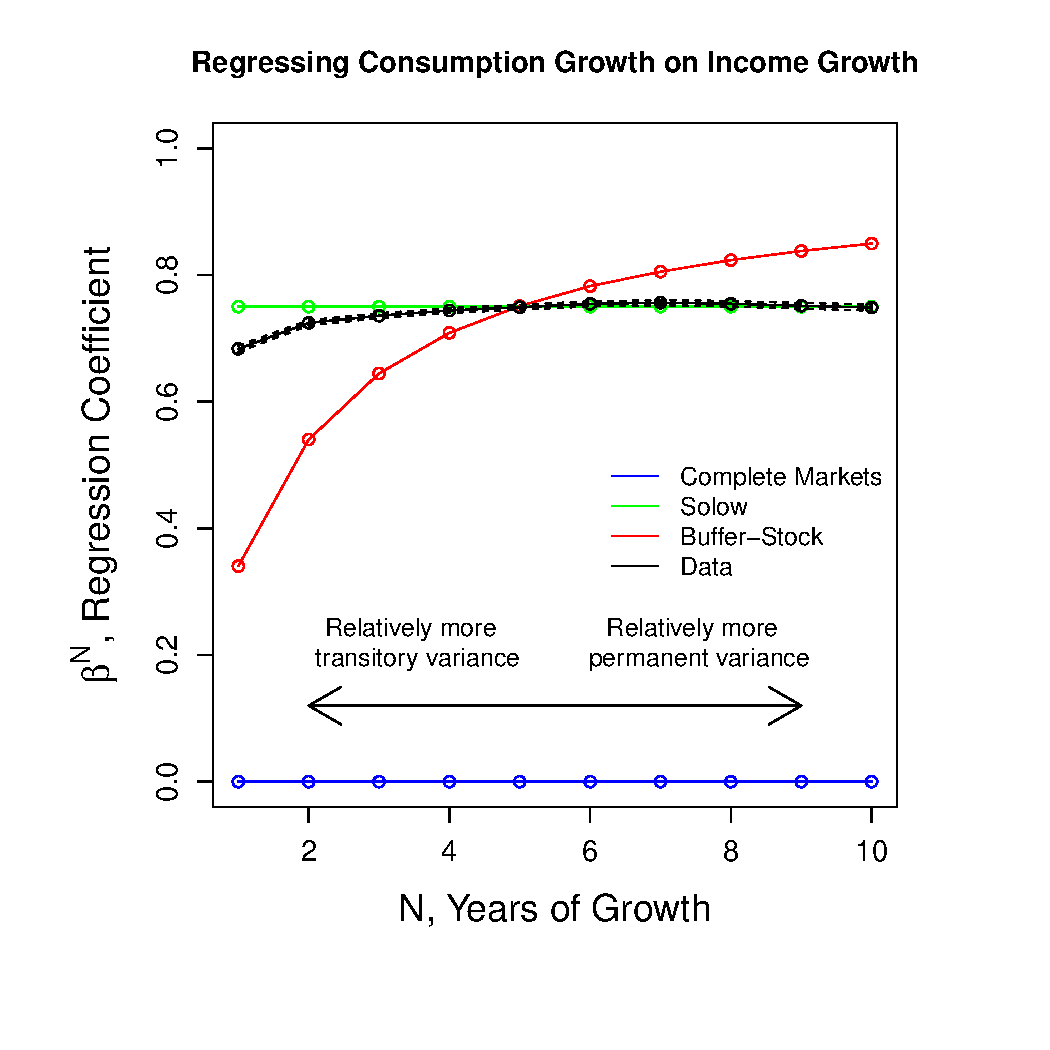
\includegraphics[height=7.5cm,trim= 0 0 0 2cm,clip]{../Figures/basic_regression_level_lincome_head.pdf}};
%	\pause
%	\node (img5) {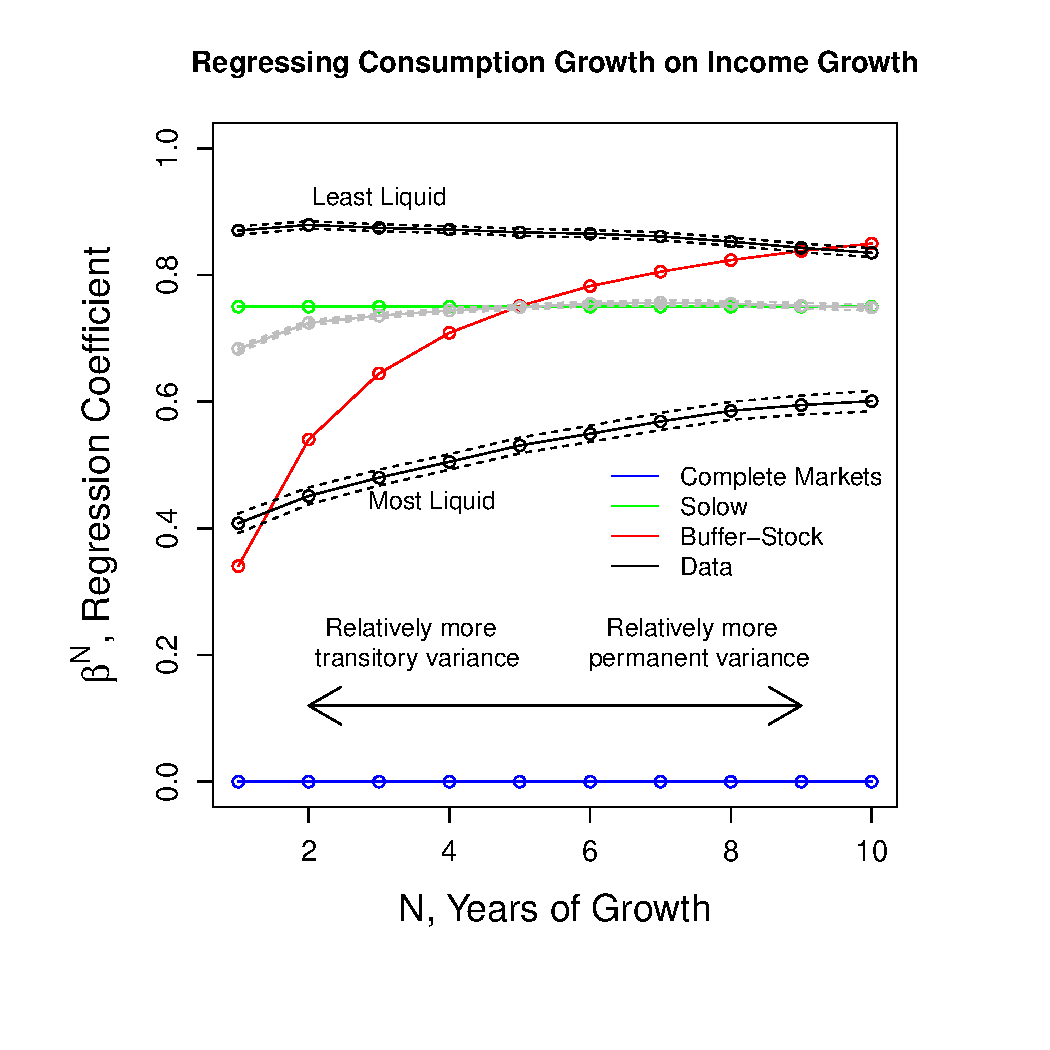
\includegraphics[height=7.5cm,trim= 0 0 0 2cm,clip]{../Figures/basic_regression_liquid_wealth_level_lincome_head.pdf}};
%	\onslide<1->
%	\end{tikzpicture}
%}
\frame
{
	\frametitle{Identification Restrictions: Income Process}
	\begin{itemize} 
		\item Permanent Income (random walk)
		\item Transitory Income (persistence $<$ 2 years)
	\end{itemize}
	\begin{figure}
		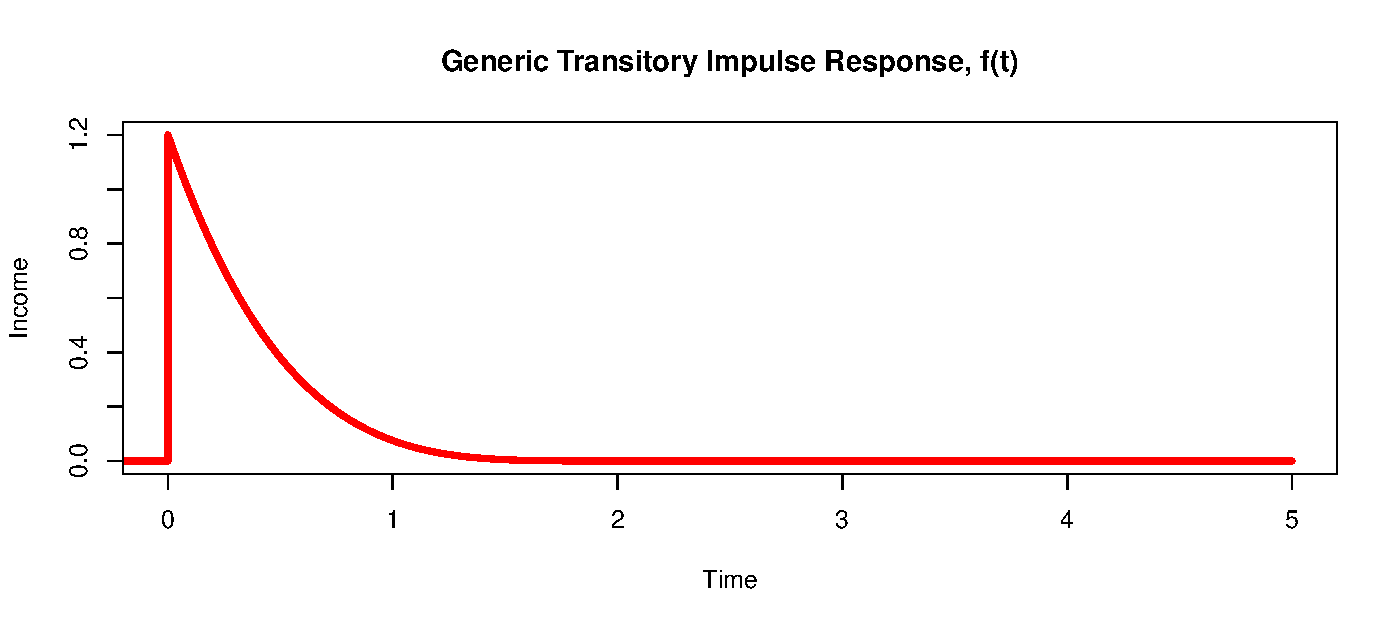
\includegraphics[scale=0.35,trim= 0 2.5cm 0 1cm]{../Figures/GenericTransitory.pdf}
	\end{figure}
	\vspace{0.5cm}
	\begin{align*}
	\onslide<2->{\color{blue} \tikz[baseline]{\node(n1){}}\bar{y}_T =} \onslide<2->{\tikz[baseline]{\node(n2){}}\int_{T-1}^{T}}\color{black} y_t\onslide<2->{\color{blue}dt} &= \onslide<2->{ \color{blue} \int_{T-1}^{T}}\color{black} \tikz[baseline]{\node(n4){}}p_t \onslide<2->{\color{blue}dt} \color{black} + \onslide<2->{\color{blue}\int_{T-1}^{T}}\color{black}\int_{t-2}^{t} \tikz[baseline]{\node(n5){}}f(t-s)dq_s\onslide<2->{\color{blue}dt}
	\end{align*}
	\only<1>{
	\begin{tikzpicture}[remember picture,overlay]
	\node (n4a)  at ([shift={(0.2,-0.05)}]n4) {};
	\node (n5a)  at ([shift={(0.5,-0.2)}]n5) {};
	\draw[blue,thick,->] (n4a)  to [in=90,out=245] + (225:1.3cm) node[anchor=north,text = blue] {Permanent income flow};
	\draw[blue,thick,->] (n5a) to [in=90,out=245] + (290:0.8cm) node[anchor=north,text = blue] {Transitory income flow};
	\end{tikzpicture}
	}
	\only<2>{
	\begin{tikzpicture}[remember picture,overlay]
	\node (n1a)  at ([shift={(0.25,0.2)}]n1) {};
	\node (n2a)  at ([shift={(0.45,-0.45)}]n2) {};
	\draw[blue,thick,->] (n1a)  to [in=270,out=90] + (90:0.6cm) node[anchor=south,text = blue] {Observed Income};
	\draw[blue,thick,->] (n2a)  to [in=90,out=270] + (270:0.6cm) node[anchor=north,text = blue] {Time Aggregation};
	\end{tikzpicture}
	}
}
\frame
{
	\frametitle{Identification Restrictions: Consumption Response}
	\label{cons_identification}
	\begin{itemize}
		\item Permanent: Moves by fraction $\phi$ of shock
		\item Transitory: Persistence $<$ 2 years \qquad \qquad \qquad \qquad \hyperlink{cons_decay}{\beamerbutton{Evidence}}
	\end{itemize}
	\begin{figure}
	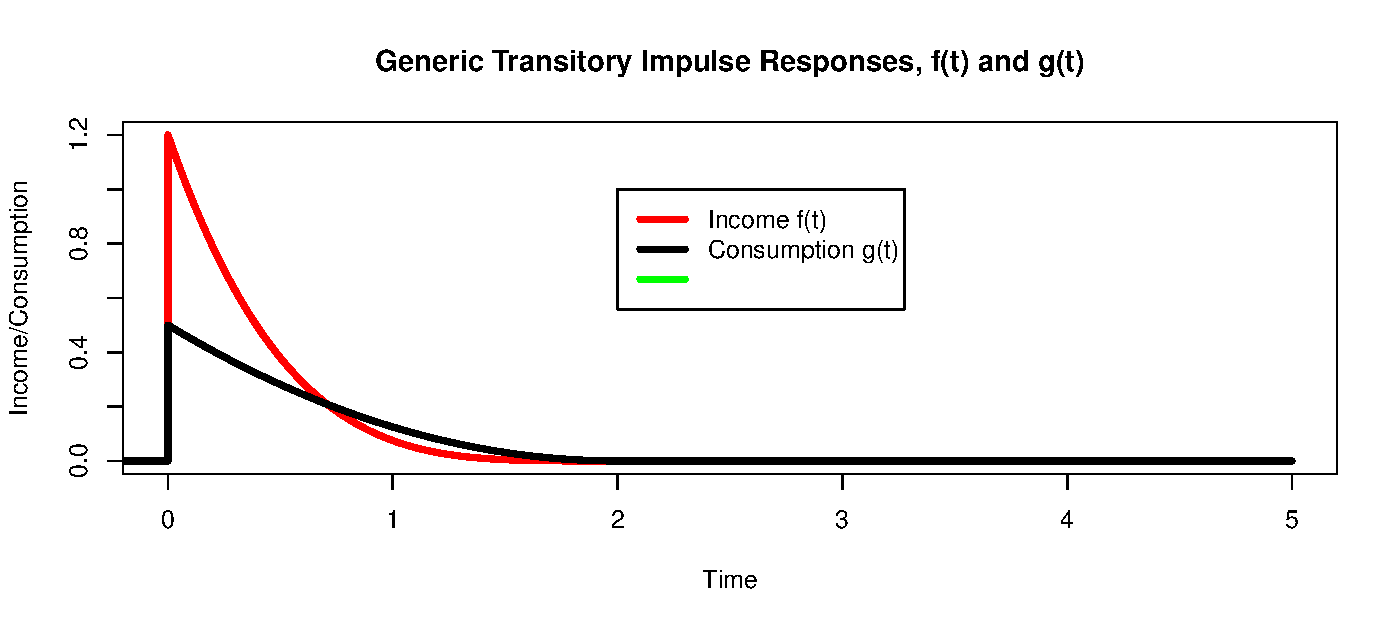
\includegraphics[scale=0.35,trim= 0 1.5cm 0 1cm]{../Figures/GenericTransitoryConsumption.pdf}
\end{figure}
\begin{align*}
\onslide<2->{\color{blue} \tikz[baseline]{\node(n1){}}\bar{c}_T =} \onslide<2->{\tikz[baseline]{\node(n2){}}\int_{T-1}^{T}}\color{black} c_t\onslide<2->{\color{blue}dt} &= \onslide<2->{ \color{blue} \int_{T-1}^{T}}\color{black} \tikz[baseline]{\node(n4){}}\phi p_t \onslide<2->{\color{blue}dt} \color{black} + \onslide<2->{\color{blue}\int_{T-1}^{T}}\color{black}\int_{t-2}^{t} \tikz[baseline]{\node(n5){}}g(t-s)dq_s\onslide<2->{\color{blue}dt}
\end{align*}
\only<1>{
	\begin{tikzpicture}[remember picture,overlay]
	\node (n4a)  at ([shift={(0.2,-0.05)}]n4) {};
	\node (n5a)  at ([shift={(0.5,-0.2)}]n5) {};
	\draw[blue,thick,->] (n4a)  to [in=90,out=245] + (225:1.3cm) node[anchor=north,text = blue] {Permanent consumption flow};
	\draw[blue,thick,->] (n5a) to [in=90,out=245] + (290:0.8cm) node[anchor=north,text = blue] {Transitory consumption flow};
	\end{tikzpicture}
}
\only<2>{
	\begin{tikzpicture}[remember picture,overlay]
	\node (n1a)  at ([shift={(0.25,0.2)}]n1) {};
	\node (n2a)  at ([shift={(0.45,-0.45)}]n2) {};
	\draw[blue,thick,->] (n1a)  to [in=270,out=90] + (90:0.6cm) node[anchor=south,text = blue] {h \ \ \ \ \ \ Observed Consumption};
	\draw[blue,thick,->] (n2a)  to [in=90,out=270] + (270:0.6cm) node[anchor=north,text = blue] {Time Aggregation};
	\end{tikzpicture}
}
}
\frame
{
	\frametitle{Full Identification}
We use GMM on the equations:
\begin{align*}
\mathrm{Var}(\Delta^N \bar{y_T} ) &=  (N-\frac{1}{3}) \sigma^2_p + 2  \sigma^2_{\tilde{q}} \\
\mathrm{Cov}(\Delta^N \bar{c_T},\Delta^N \bar{y_T} ) &= \phi (N-\frac{1}{3}) \sigma^2_p + 2 \psi \sigma^2_{\tilde{q}}
\end{align*}
with $N=3,4,5$ (and $T=2007,..,2015$) to identify:\\
\bigskip
\begin{itemize}
	\item $\sigma^2_p$: Permanent shock variance
	\item $\sigma^2_{\tilde{q}}$: (Time aggregated) transitory shock variance
	\item $\phi$: MPX out of permanent income shocks
	\item $\psi$: MPX out of transitory income shocks
\end{itemize}
\bigskip
where  $\psi$ is the regression coefficient of `transitory' consumption on transitory income
\hyperlink{whynotbpp}{\beamerbutton{Why not BPP}}
}


\section{Data}
\frame
{
	\frametitle{Data}
	What we need:
	\begin{itemize}
		\item Panel Data on \textbf{Income} and \textbf{Expenditure}
		\item Household \textbf{Balance Sheets} 
	\end{itemize}
	\bigskip
	\pause
	What we have: Registry data for all Danish households
	\begin{itemize}
		\item \textbf{Income}
		\begin{itemize}
			\item[] Third party reported
			\item[] After-tax, restrict to heads aged 30-55
		\end{itemize}
		\item \textbf{Balance Sheet}
		\begin{itemize}
			\item[] Wealth on 31 Dec
			\item[] Asset category, mortgage tenure
		\end{itemize}
	\item \textbf{Expenditure}
		\begin{itemize}
		\item[] No \textit{direct} measure of spending
		\end{itemize}
	\end{itemize}
}
\frame[t]
{
	\frametitle{Data: Expenditure}
	\label{data_expenditure}
	Intertemporal budget constraint
		\begin{align*}
			\text{Expenditure} \qquad = \qquad \tikz[baseline]{\node(income){}}\text{Income}\qquad  - \qquad \tikz[baseline]{\node(saving){}}\text{Saving}
		\end{align*}
		\bigskip
	\only<2->{
	\begin{tikzpicture}[remember picture,overlay]
	\node (incomea)  at ([shift={(0.6,-0.1)}]income) {};
	\node (incomeb)  at ([shift={(0,-0.4)}]incomea) {};
	\node (savinga)  at ([shift={(0.6,-0.1)}]saving) {};
	\node (savingb)  at ([shift={(0,-0.4)}]savinga) {};
	%\draw[blue,thick,->] (incomea)  to [in=90,out=-90] (incomeb) node[anchor=north,text = blue] {\begin{tabular}{l} Known  \end{tabular}};
	\draw[blue,thick,->] (savinga)  to [in=90,out=-90] (savingb) node[anchor=north,text = blue] {\begin{tabular}{r} = Change in Net Worth \  \\ (adj. for capital gains)  \end{tabular}};
	\end{tikzpicture}
	}
	\only<3->{
	\begin{itemize}
		\item Works well for households with simple financial lives
		\item Problem: Capital gains
		\begin{itemize}
			\item[] Houses off balance sheet (exclude transaction years)
			\item[] Exclude business owners
			\item[] Capital gains based on a diversified index
		\end{itemize}
		\item Noisy, but perhaps better than surveys (Kuchler et al. 2018)
		\item Huge sample size advantage: sample covers 7.6 million observations over 2004-2015
	\end{itemize}
	\hyperlink{summary_stats}{\beamerbutton{Summary Statistics}}
	\hyperlink{measurementerror}{\beamerbutton{On measurement error}}
	}
}


\section{Liquid Wealth}
\frame
{
	\frametitle{Results by Liquid Wealth}
	\label{MPXbyLiquidWealth}
	\begin{columns}
		\column{0.5\linewidth}
		\centering
		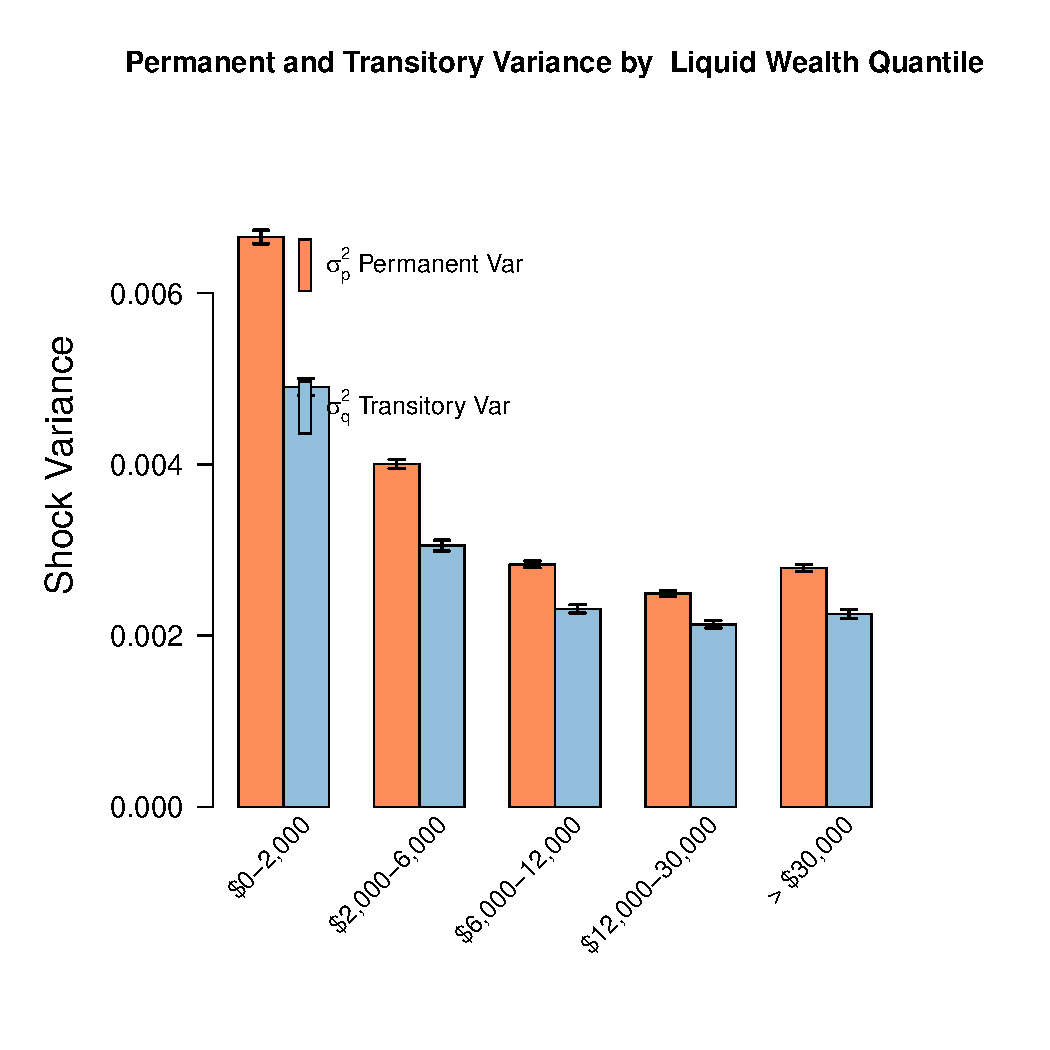
\includegraphics[scale=0.35]{../Figures/VarianceByLiquidWealth_level_lincome_head.pdf}
		\column{0.5\linewidth}
		\centering
		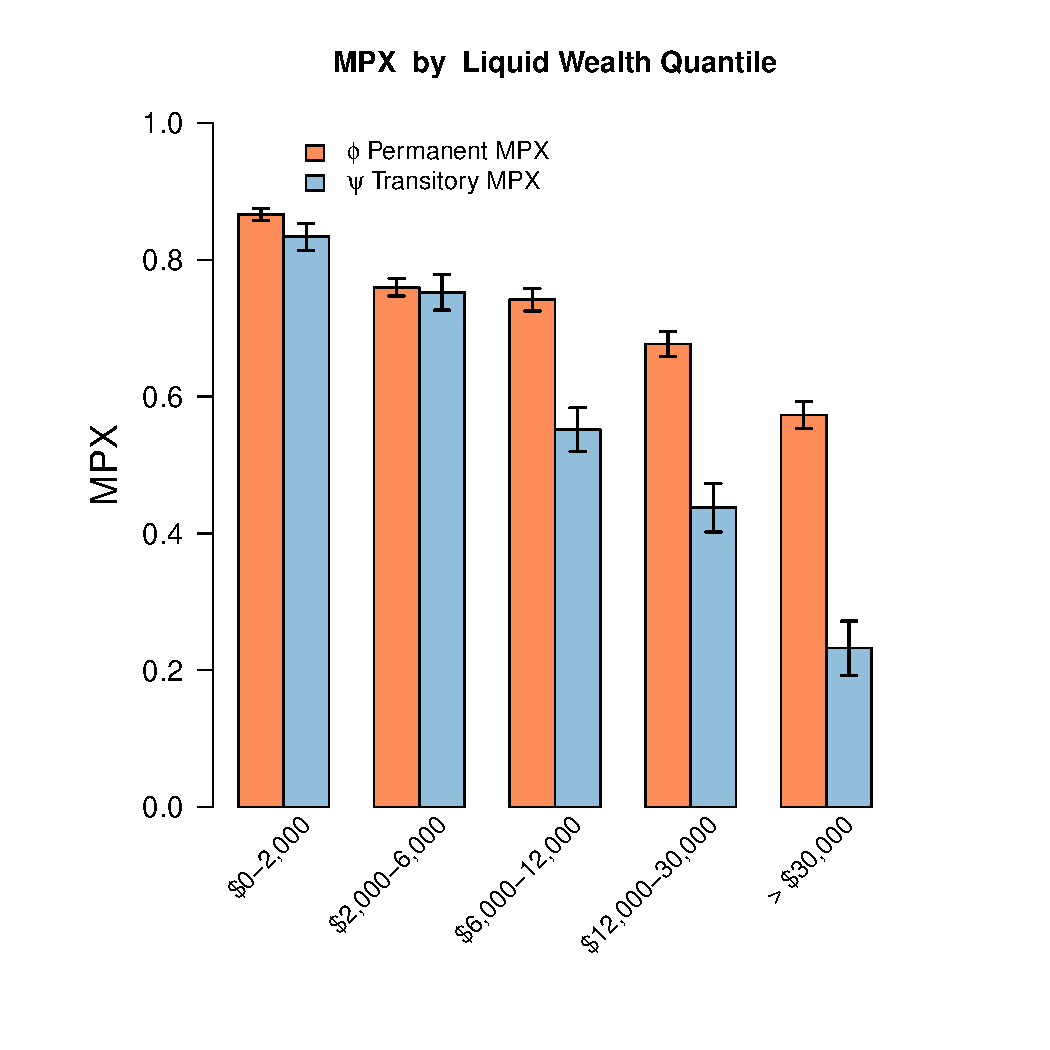
\includegraphics[scale=0.35]{../Figures/MPXByLiquidWealth_level_lincome_head.pdf}
	\end{columns} 
	\hyperlink{MPXbyNetWealth}{\beamerbutton{MPX by Net Wealth}}	
}

\section{Monetary Policy}
\frame{
	\frametitle{Monetary Policy: Auclert's Decomposition}
	How does Monetary Policy Effect Aggregate Consumption?\\
	\bigskip
	\begin{itemize}
		\item Intertemporal Substitution \tikz[baseline]{\node(topbrace1){}}
		\item Aggregate Income \tikz[baseline]{\node(bottombrace1){}}
	\begin{tikzpicture}[overlay, remember picture]
	\draw [decoration={brace,amplitude=0.5em},decorate,ultra thick,black]
	let \p1=(topbrace1), \p2=(bottombrace1) in
	({max(\x1,\x2)+1.8em}, {\y1+0.8em}) -- node[right=0.6em] {Representative Agent Channels} ({max(\x1,\x2)+1.8em}, {\y2});
	\end{tikzpicture}
	\pause
	\only<2>{
	\begin{tikzpicture}[remember picture,overlay]
	\node (topbrace1a)  at ([shift={(-5,0.1)}]topbrace1) {};
	\node (topbrace1b)  at ([shift={(-5,1.8)}]topbrace1) {};
	\node (bottombrace1a)  at ([shift={(-3.7,0.1)}]bottombrace1) {};
	\node (bottombrace1b)  at ([shift={(-3.7,-0.7)}]bottombrace1) {};
	\draw[blue,thick,->] (topbrace1a)  to [in=180,out=180] (topbrace1b) node[anchor=west,text = blue] {Dominates in Rep. Agent NK models};
	\draw[blue,thick,->] (bottombrace1a)  to [in=180,out=180] (bottombrace1b) node[anchor=west,text = blue] {Large in Spender-Saver, or TANK models};
	\end{tikzpicture}
	}
		\pause
		\item Fisher (Inflationary debt relief) \tikz[baseline]{\node(topbrace2){}}
		\item Earnings Heterogeneity
		\item Interest Rate Exposure \tikz[baseline]{\node(m1){}}
	\begin{tikzpicture}[overlay, remember picture]
\draw [decoration={brace,amplitude=0.5em},decorate,ultra thick,black]
let \p1=(topbrace2), \p2=(m1) in
({max(\x1,\x2)}, {\y1+0.8em}) -- node[right=0.6em] {Redistribution Channels} ({max(\x1,\x2)}, {\y2});
\end{tikzpicture}
	\end{itemize}
	\bigskip
	\pause
	How can we \textit{empirically} measure the size of the redistribution channels?\\
	\bigskip
	Need to know the distribution of MPCs along the relevant dimension of redistribution
}
\frame{
	\frametitle{Interest Rate Exposure: Auclert's Experiment}
	\textbf{Key assumption:} \\Households treat redistribution like an income shock\\
	\pause
	\bigskip
	\textbf{Experiment}
	\begin{itemize}
		\item[] Short term real interest rate $\uparrow$ 1\% for 1 year
		\item[] Hold constant income and inflation
	\end{itemize}
	\bigskip
	How does subsequent \textbf{redistribution} impact \textbf{aggregate consumption}?\\
	\bigskip
	Dimension of Redistribution: \textbf{Unhedged Interest Rate Exposure}
}
\frame{
	\frametitle{Interest Rate Exposure: Dimension of Redistribution}
	Define \textbf{Unhedged Interest Rate Exposure} for household $i$ as the total savings the household will invest at this year's interest rate:
	\begin{align*}
	URE_i = Y_i - C_i + A_i - L_i
	\end{align*}
	Where
	\begin{itemize}
		\item $Y_i = $ Total after tax income 
		\item $C_i = $ Total Expenditure, including interest payments
		\item $A_i = $ Maturing assets
		\item $L_i = $ Maturing liabilities
	\end{itemize}
	Following a change in the interest rate $dR$, the size of the Interest Rate Exposure channel on household $i$'s expenditure is:
	\begin{align*}
		dc_i = MPC_i URE_i  \frac{dR}{R}
	\end{align*}
}
\frame{
	\frametitle{Interest Rate Exposure: Aggregation}
	\label{aggregation}
	Aggregate to find size of channel:
	\begin{align*}
	dc_i &= \quad \ \ MPC_i URE_i  \ \ \ \frac{dR}{R} \\
	\implies \frac{dC}{C} &= \mathbb{E}_I \Big(MPC_i \frac{URE_i}{\mathbb{E}_I (c_i)}   \Big) \frac{dR}{R} 
	\end{align*}
	Define sufficient statistic:
	\begin{align*}
	\mathcal{E}_R  = \mathbb{E}_I \Big(MPC_i \frac{URE_i}{\mathbb{E}_I (c_i)}   \Big) 
	\end{align*}
	\bigskip
	$\implies$ Need to know the distribution of $MPC_i$ with $URE_i$\\
	\bigskip
	We can do that! \hspace{4.9cm} \hyperlink{OutOfSample}{\beamerbutton{Out of Sample Assumptions}}
}
\frame{
	\frametitle{Interest Rate Exposure: MPX Distribution}
		\begin{center}
		\begin{tikzpicture}
%		\node (img1) {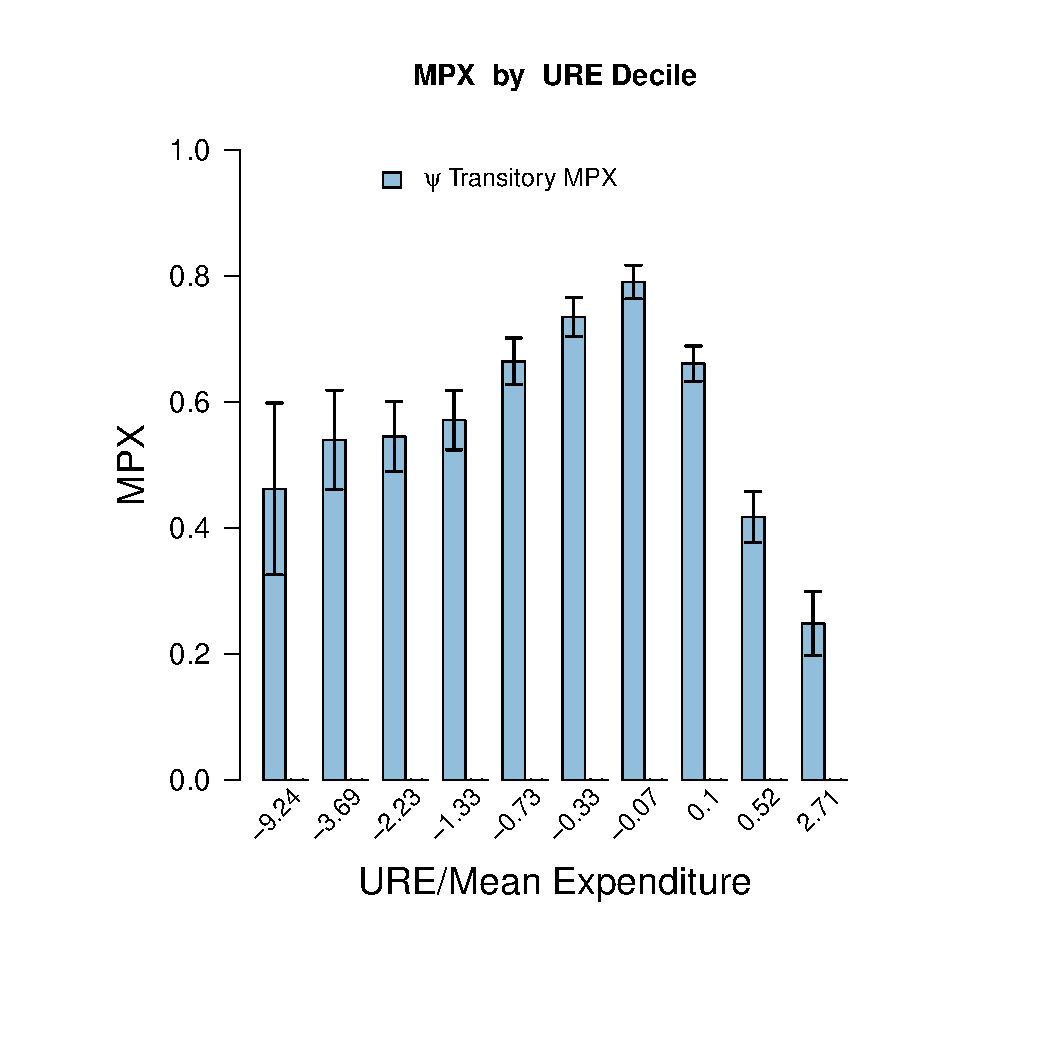
\includegraphics[scale=0.5]{../Figures/MPXByUREdetails1_level_lincome_head.pdf}};
%		\pause
		\node (img2) {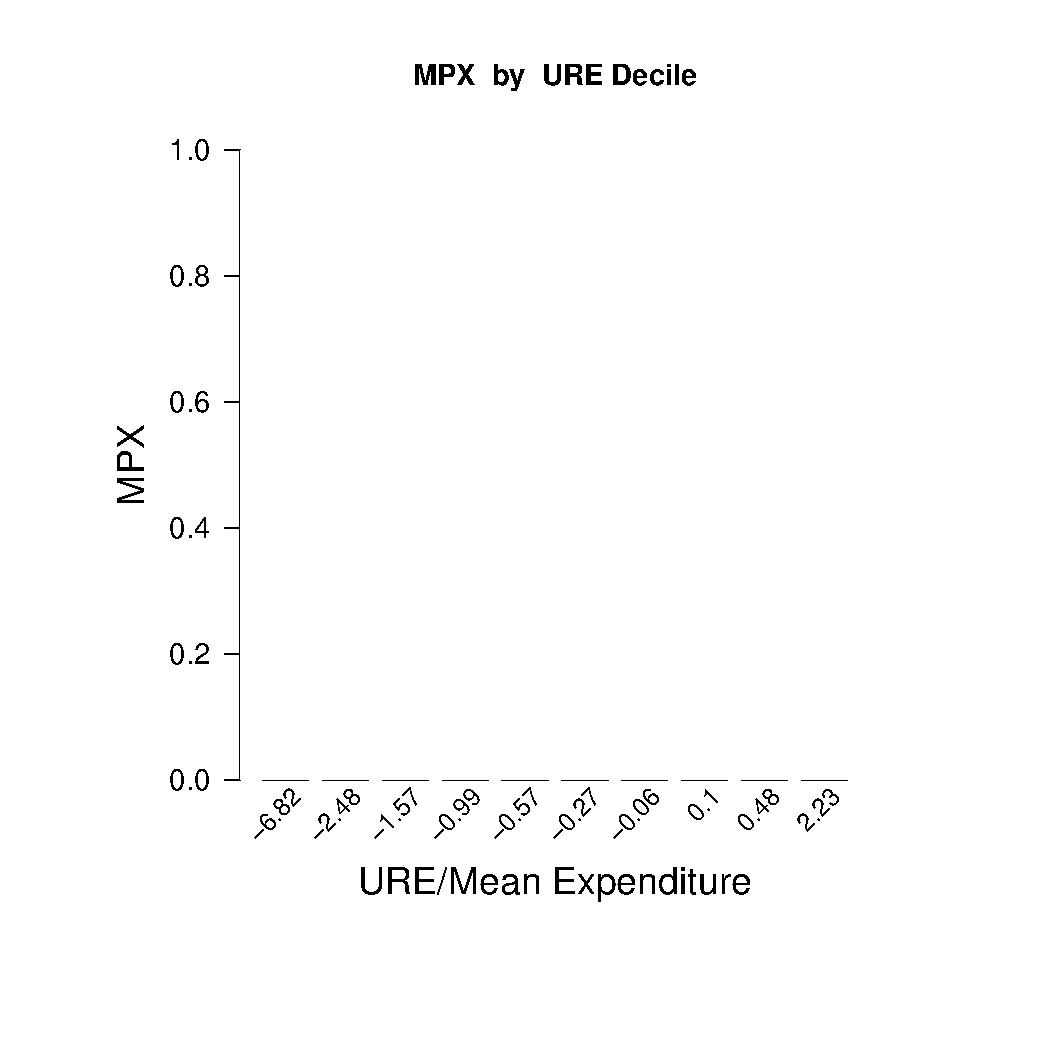
\includegraphics[scale=0.5]{../Figures/MPXByUREdetailsblank_level_lincome_head.pdf}};
		\node (img3)
		{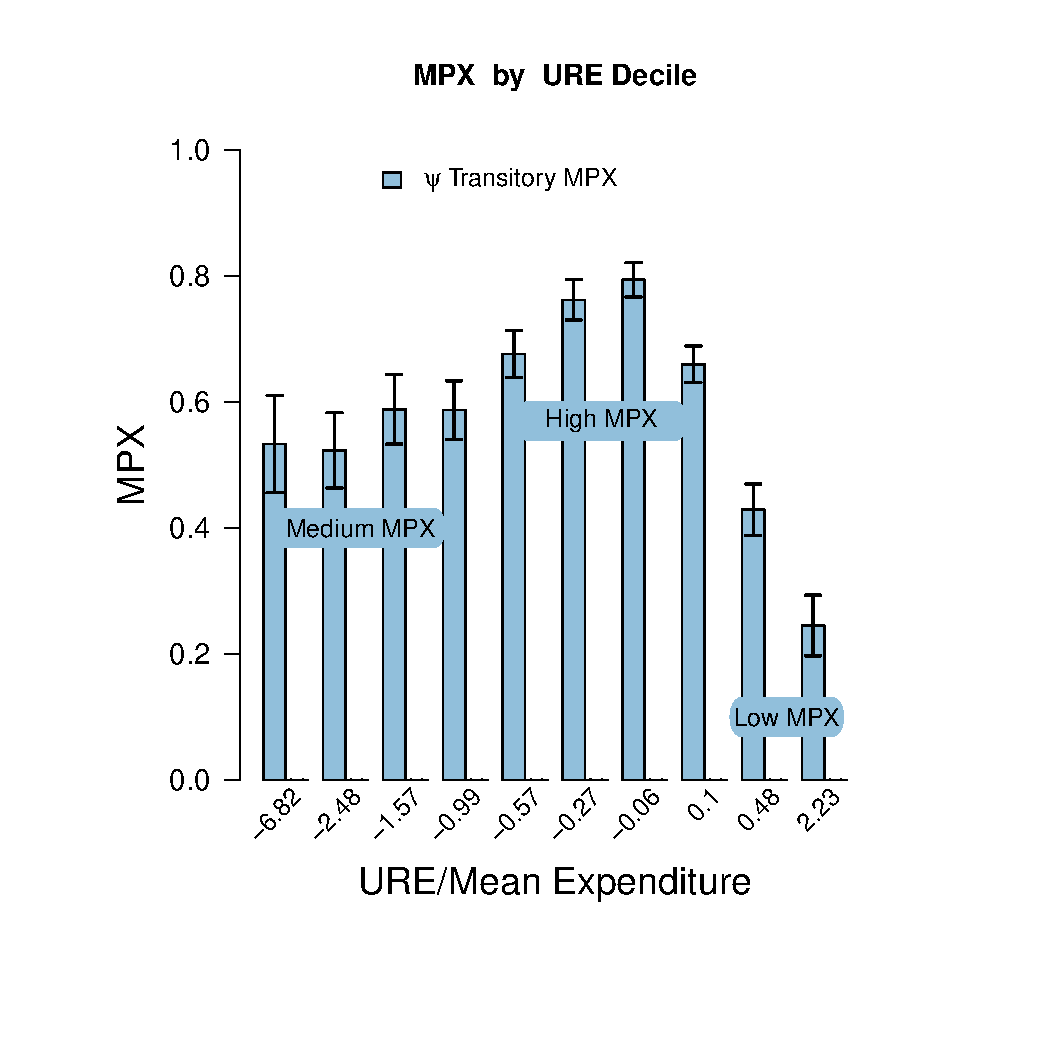
\includegraphics[scale=0.5]{../Figures/MPXByUREdetails1a_level_lincome_head.pdf}};
%		\pause
%		\node (img4) {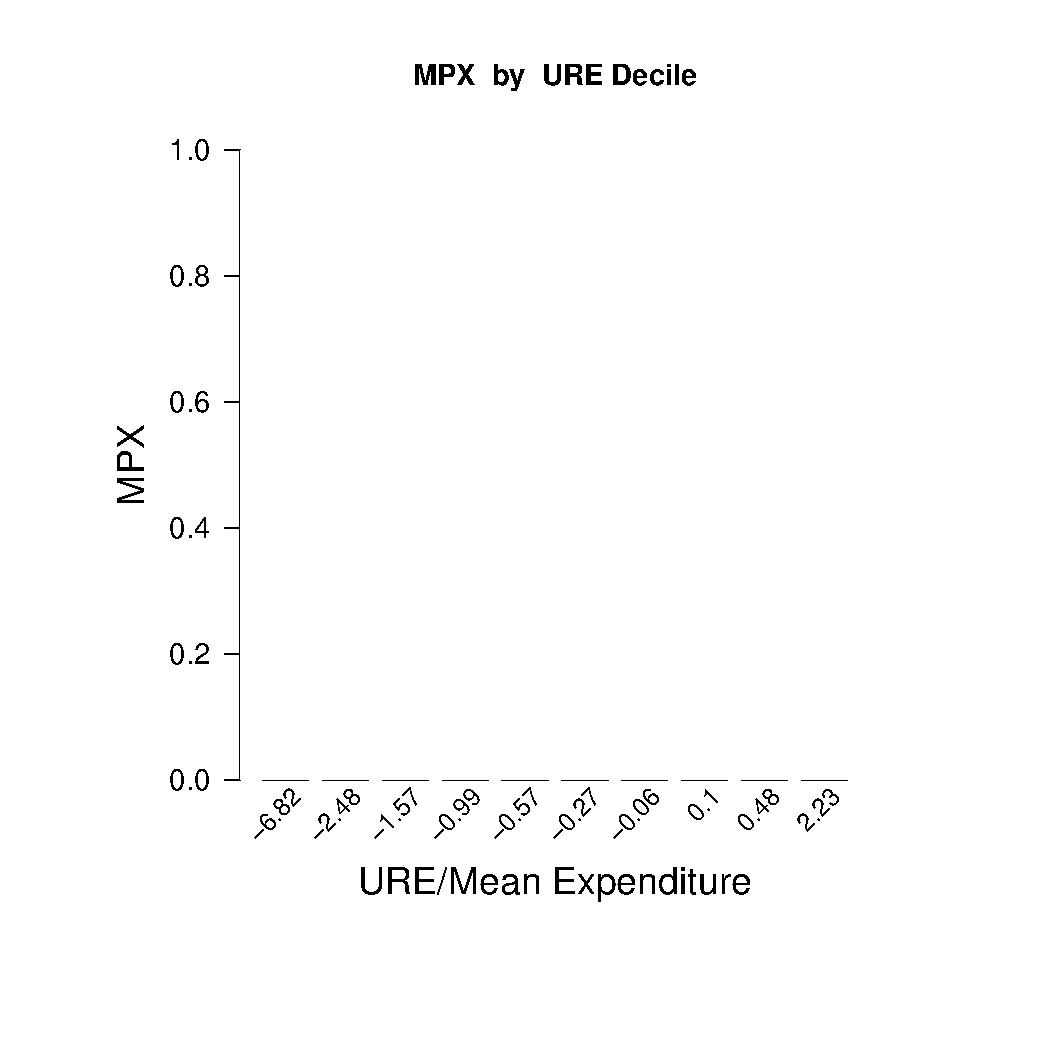
\includegraphics[scale=0.5]{../Figures/MPXByUREdetailsblank_level_lincome_head.pdf}};
%		\node (img5) {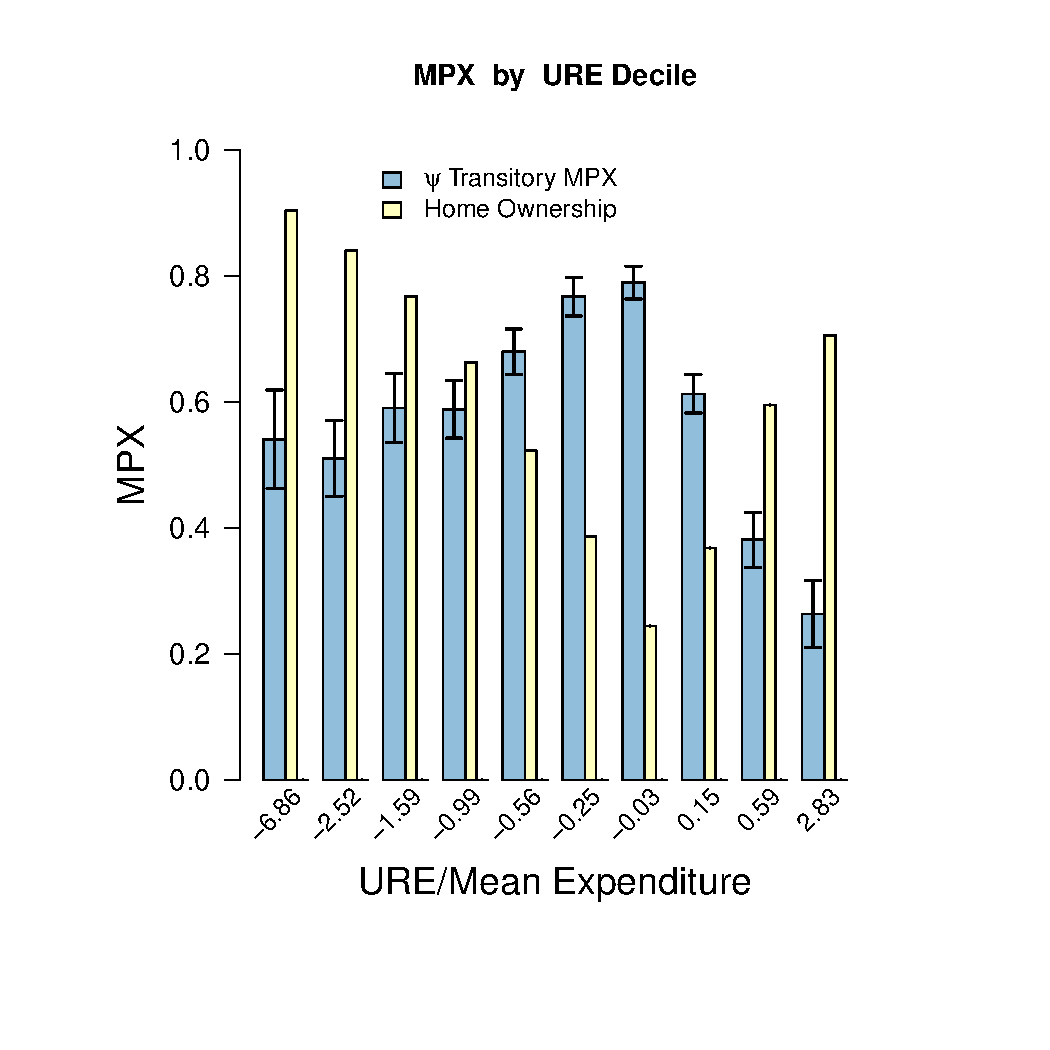
\includegraphics[scale=0.5]{../Figures/MPXByUREdetails2_level_lincome_head.pdf}};
		\pause
		\node (img6) {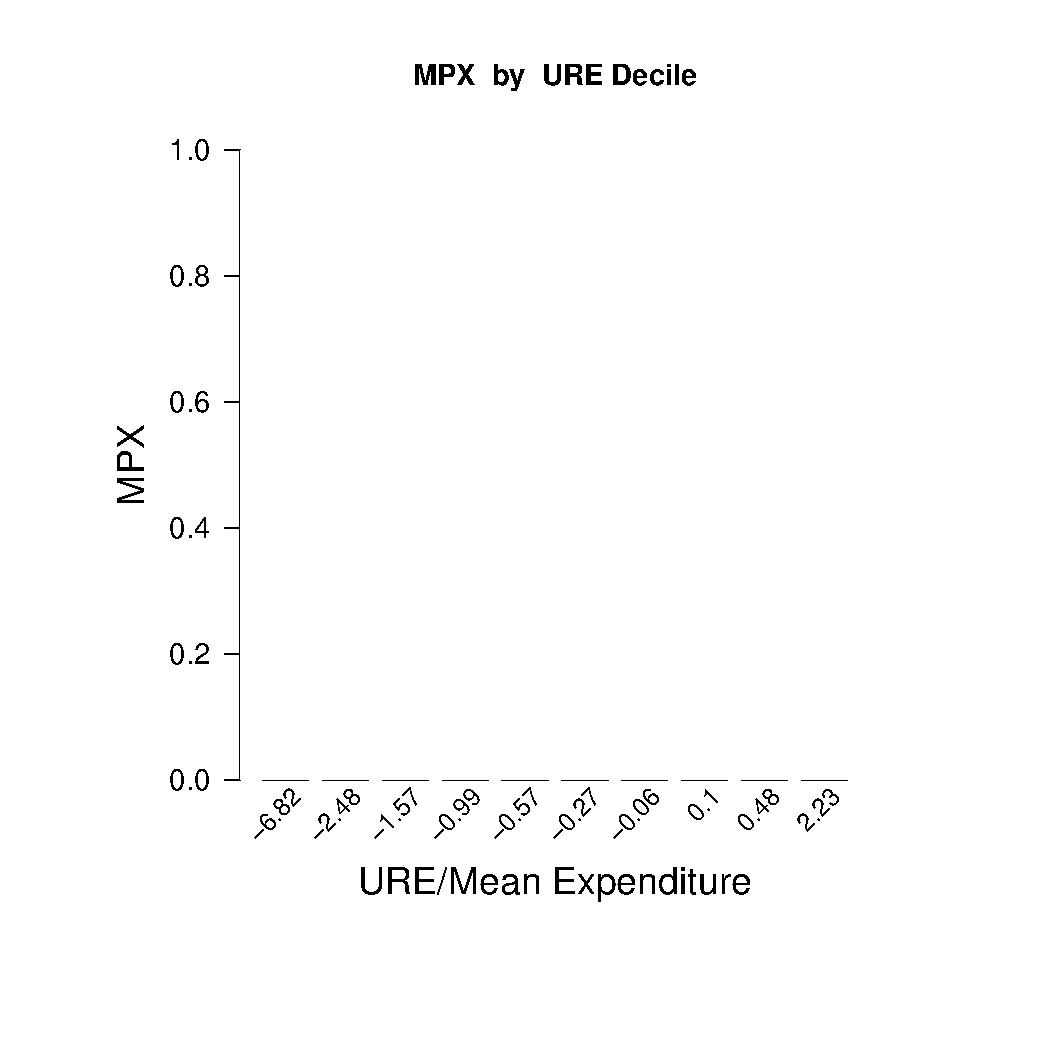
\includegraphics[scale=0.5]{../Figures/MPXByUREdetailsblank_level_lincome_head.pdf}};
		\node (img7)
		{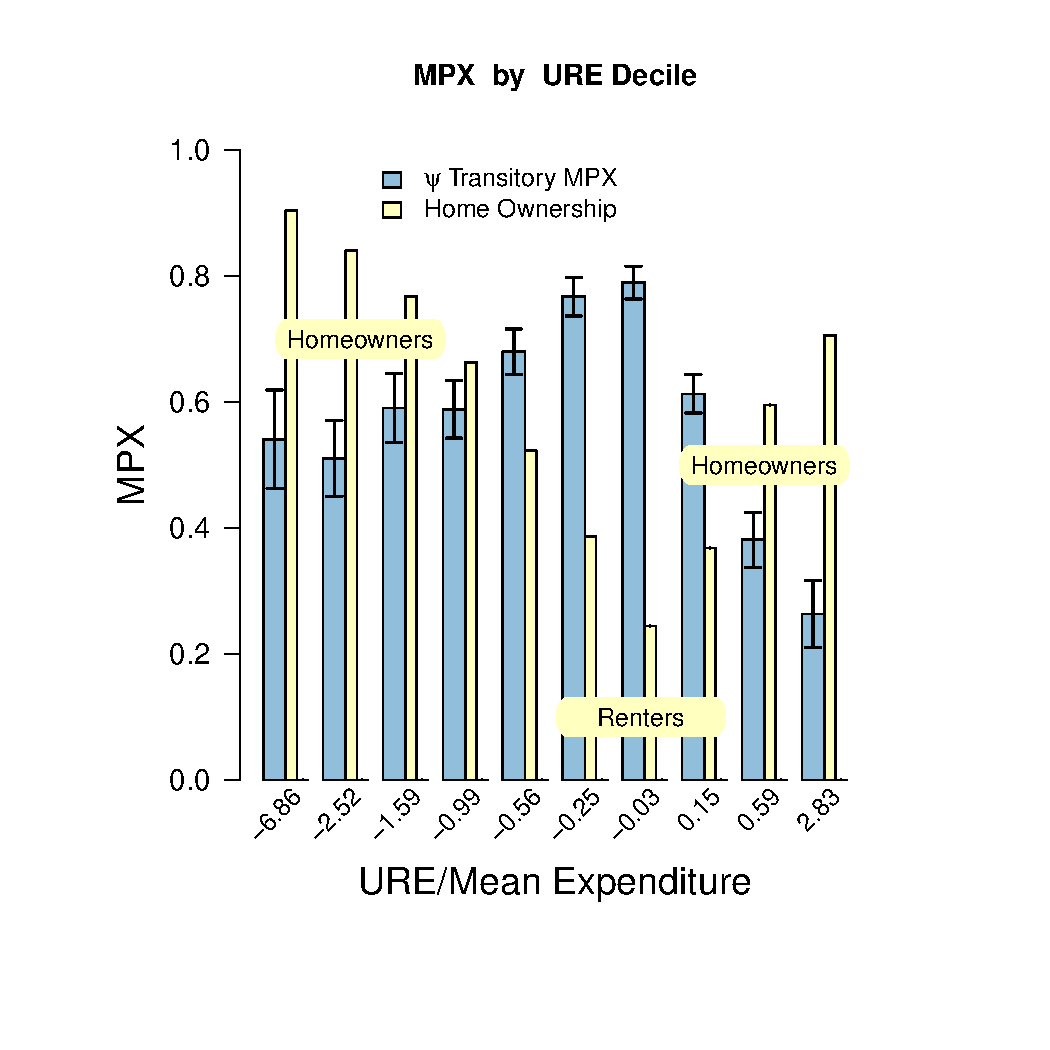
\includegraphics[scale=0.5]{../Figures/MPXByUREdetails2a_level_lincome_head.pdf}};
%		\pause
%		\node (img8) {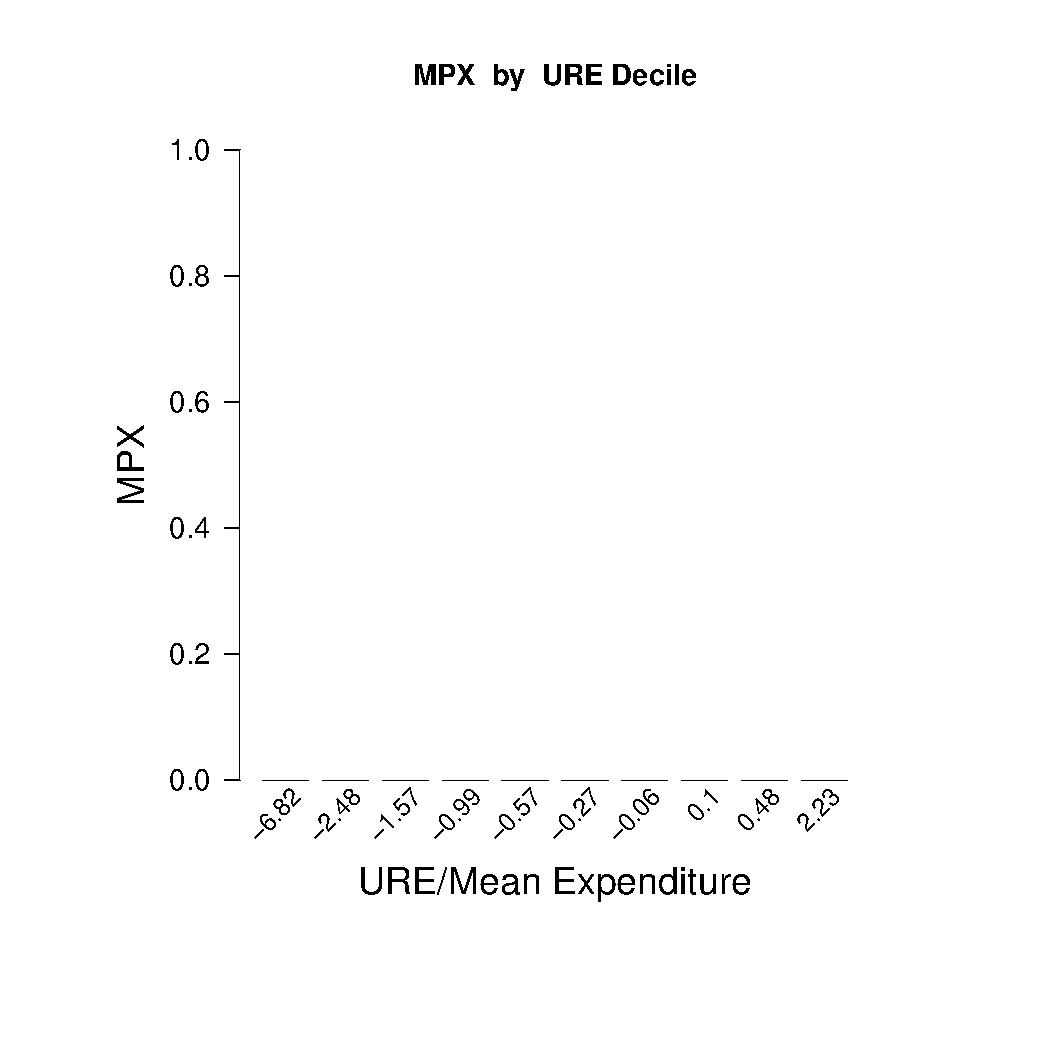
\includegraphics[scale=0.5]{../Figures/MPXByUREdetailsblank_level_lincome_head.pdf}};
%		\node (img9) {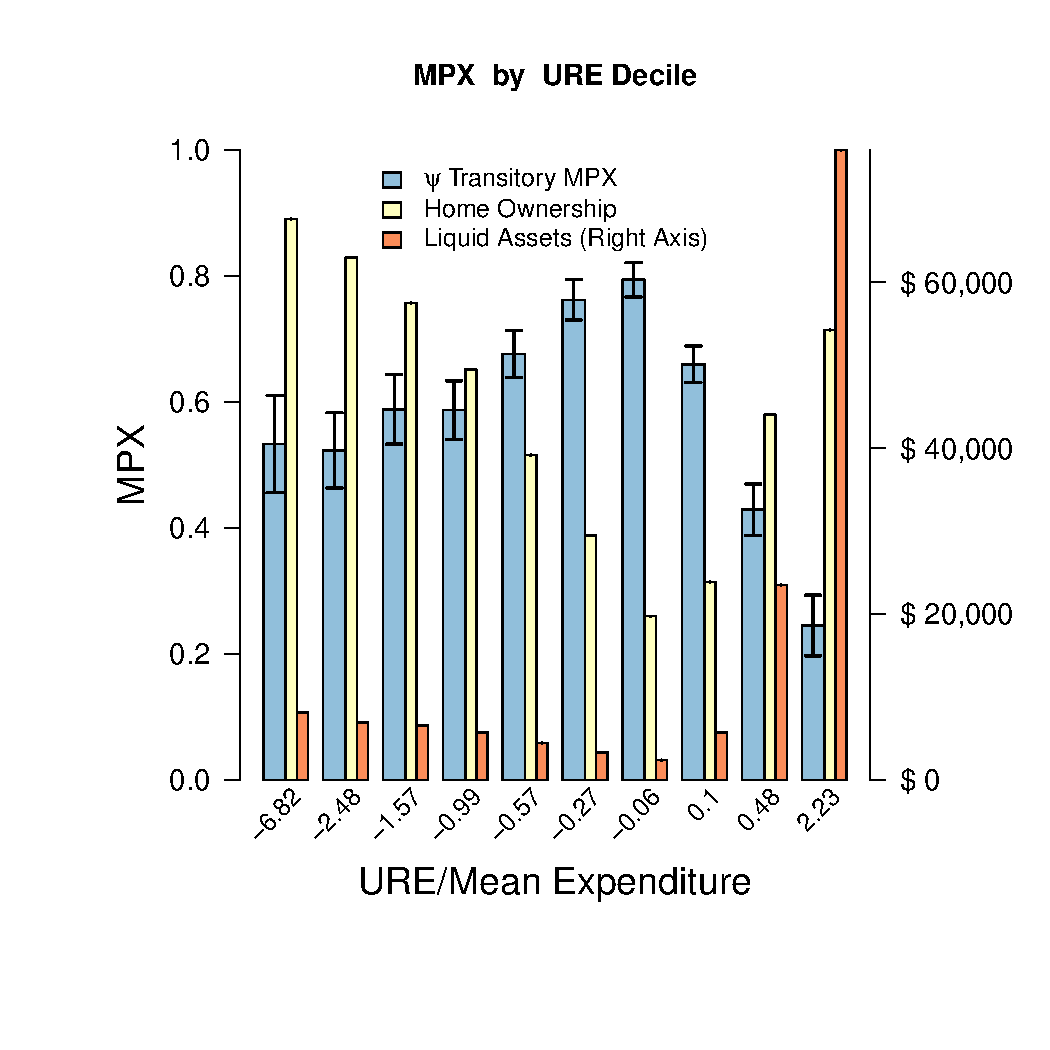
\includegraphics[scale=0.5]{../Figures/MPXByUREdetails3_level_lincome_head.pdf}};
		\pause
		\node (img10) {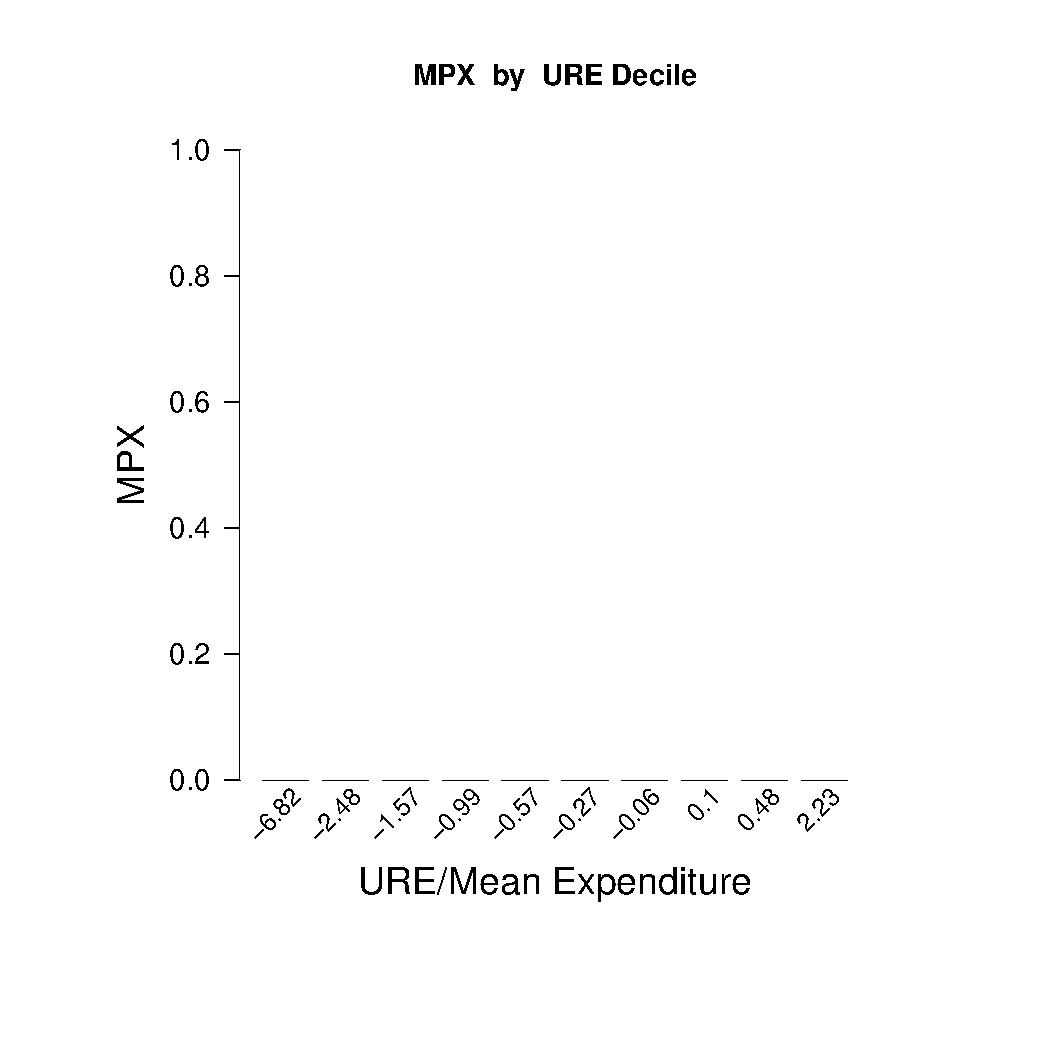
\includegraphics[scale=0.5]{../Figures/MPXByUREdetailsblank_level_lincome_head.pdf}};
		\node (img11) {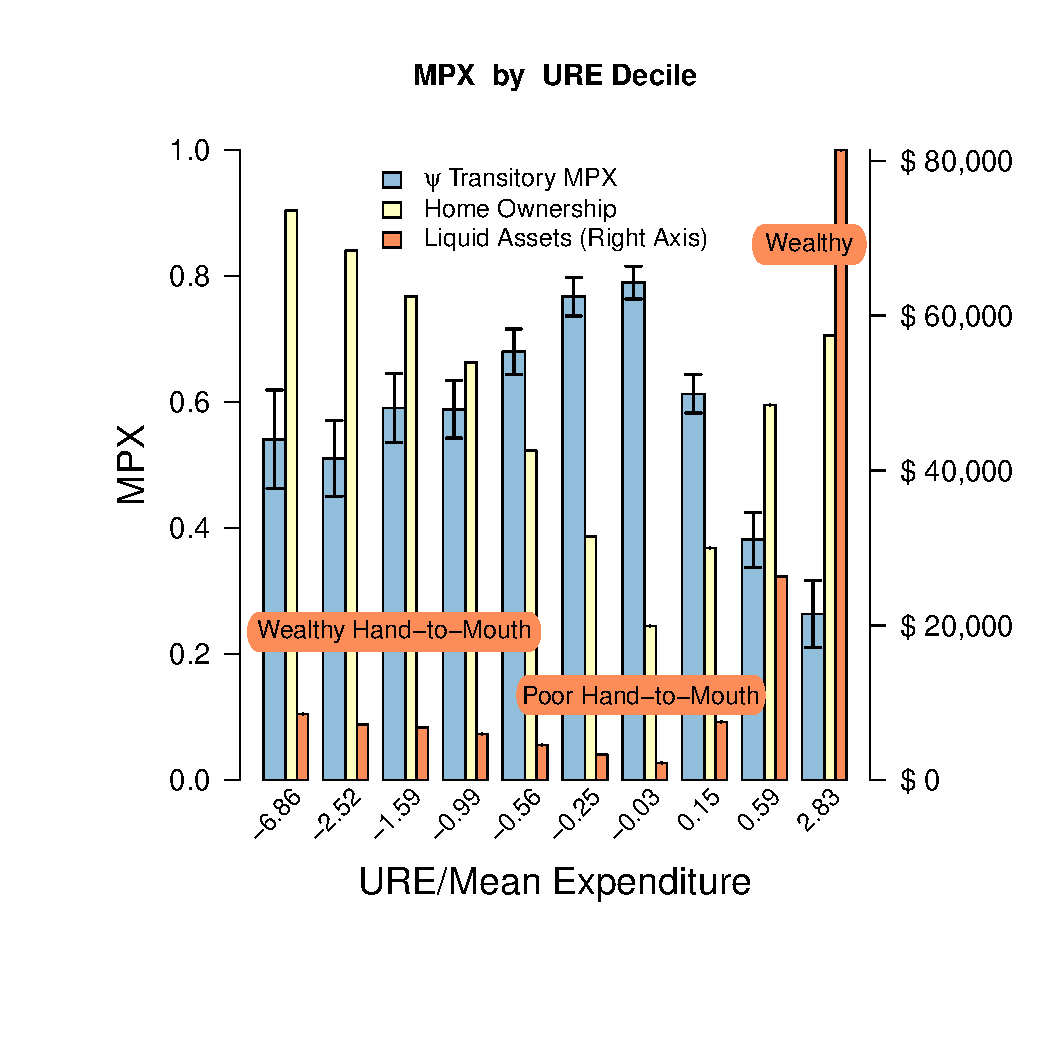
\includegraphics[scale=0.5]{../Figures/MPXByUREdetails3a_level_lincome_head.pdf}};
		\onslide<1->
		\end{tikzpicture}
	\end{center}
}
\frame{
	\frametitle{Interest Rate Exposure: Out of Sample}
	\textit{Total} URE sums to zero - this is not true for our household sample 
	\begin{itemize} 
		\item -61bn USD 
	\end{itemize}
	\bigskip
	\tiny
	\input ../Tables/URE_table.tex
}
\frame{
	\frametitle{All Five Transmission Channels}
	\begin{align*} 
	\frac{dC}{C} &= \overbrace{\mathcal{M}\frac{dY}{Y}}^{\text{Aggregate Income Channel}\qquad} \overbrace{ + \gamma \mathcal{E}_Y \frac{dY}{Y}}^{\text{Earnings Heterogeity Channel}\qquad} \overbrace{ - \mathcal{E}_P\frac{dP}{P}}^{\text{Fisher Channel}}  \nonumber \\
	& \qquad \underbrace{ + \mathcal{E}_R \frac{dR}{R}}_{\text{Interest Rate Exposure Channel}\qquad}  \underbrace{ - \sigma \mathcal{S}\frac{dR}{R}}_{\text{Intertemporal Substitution Channel}} \label{auclert_channels}
	\end{align*}
	\begin{columns}
	\column{0.5\linewidth}
	\centering
		\input ../Tables/sufficient_stats2.tex
	\column{0.5\linewidth}
	\pause
	Compare $\mathcal{E}_R$ to $\sigma S$:\\
	\bigskip
	$\sigma \approx 0.1$ Best, Cloyne, Ilzetzki, and Kleven (2019)\\
	\bigskip
	 $\sigma S \approx 0.05$ \\
	\end{columns}

	\begin{tikzpicture}[remember picture,overlay]
	\draw[red,thick] (2.84,0.87) circle (0.45cm);
	\draw[red,thick] (7.1,0.51) circle (0.45cm);
	\end{tikzpicture} 
}
\section{Model}
\frame{
	\frametitle{Aim of Modeling Exercise}
	Can we calibrate a standard Buffer-Stock saving model to fit the distribution of MPC with liquid wealth?
	\begin{columns}
	\column{0.5\linewidth}
	\centering
	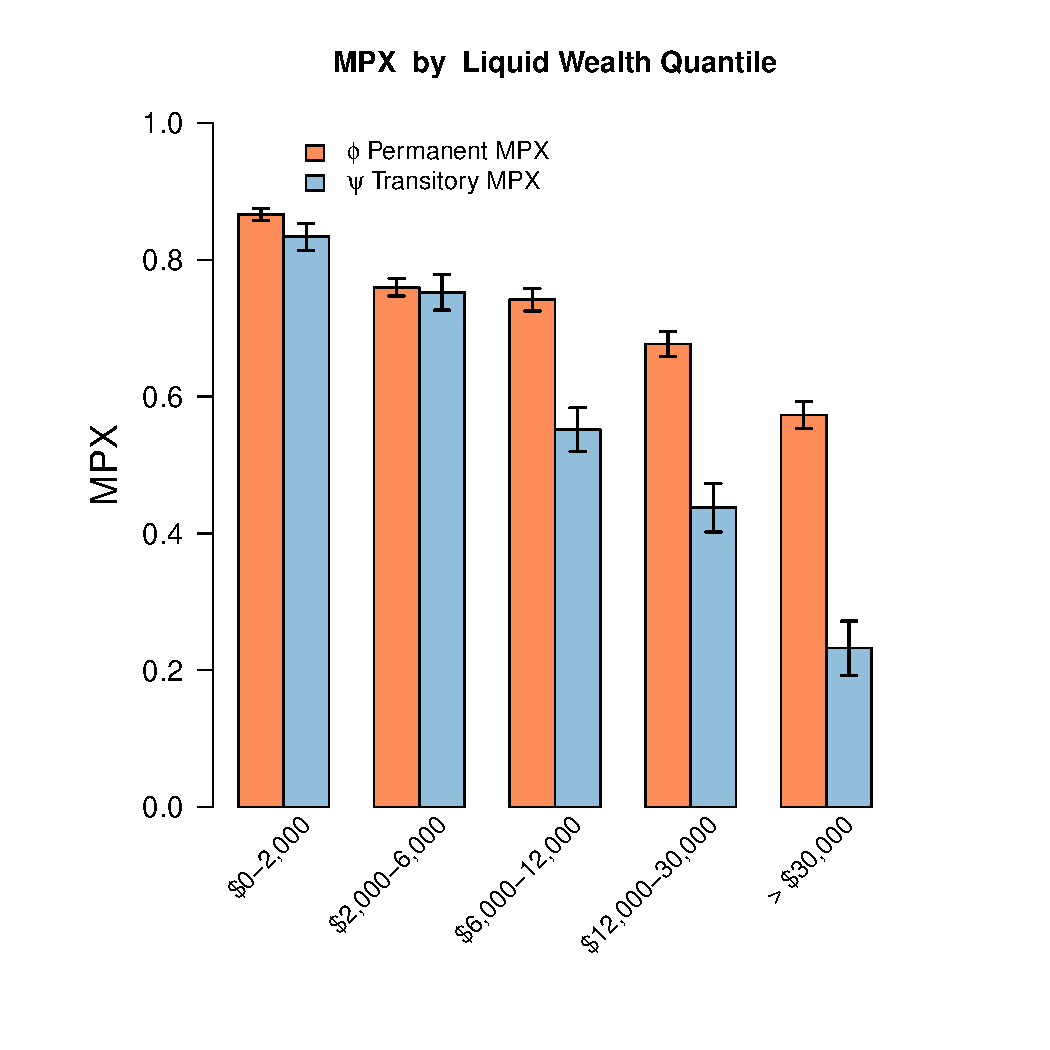
\includegraphics[scale=0.35]{../Figures/MPXByLiquidWealth_level_lincome_head.pdf}
	\column{0.5\linewidth}
	Key features:
	\begin{itemize}
		\item High overall Transitory MPC
		\item Decreasing with liquid wealth
	\end{itemize}
\end{columns}
}
\begin{comment}

\frame{
	\frametitle{Benchmark Model}
	Households maximize expected utility
	\begin{align*}
	\mathbb{E}_t \sum_{i=t}^{\infty} \beta^i u(\cLevBF_i)
	\end{align*}
	with:
	\begin{itemize}
		\item Permanent and Transitory shocks to income (calibrated to Danish data)
		\item Saving in one (liquid) asset
		\item No borrowing
		\item CRRA utility, $\rho = 2$
	\end{itemize}
}
\frame{
	\frametitle{Benchmark Model: Fitting the Liquid Wealth Distribution}
	Ex-ante heterogeneity in the discount rate\\
	\bigskip
	$\beta^i \sim \text{Unif}[ \beta_{\text{low}}, \beta_{\text{high}} ]$ Chosen to fit level and distribution of liquid wealth (especially at the low end)\\
	\centering
	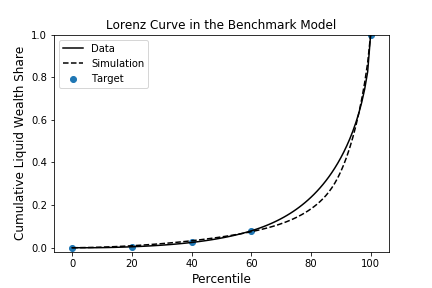
\includegraphics[scale=0.45]{../Figures/benchmark_Lorenz.png}	
}
\frame{
	\frametitle{Benchmark Model: Results}
	Simulate panel of data and estimate $\phi$ and $\psi$
	\begin{columns}
	\column{0.5\linewidth}
	\centering
	\begin{tikzpicture}
	\node (img1) {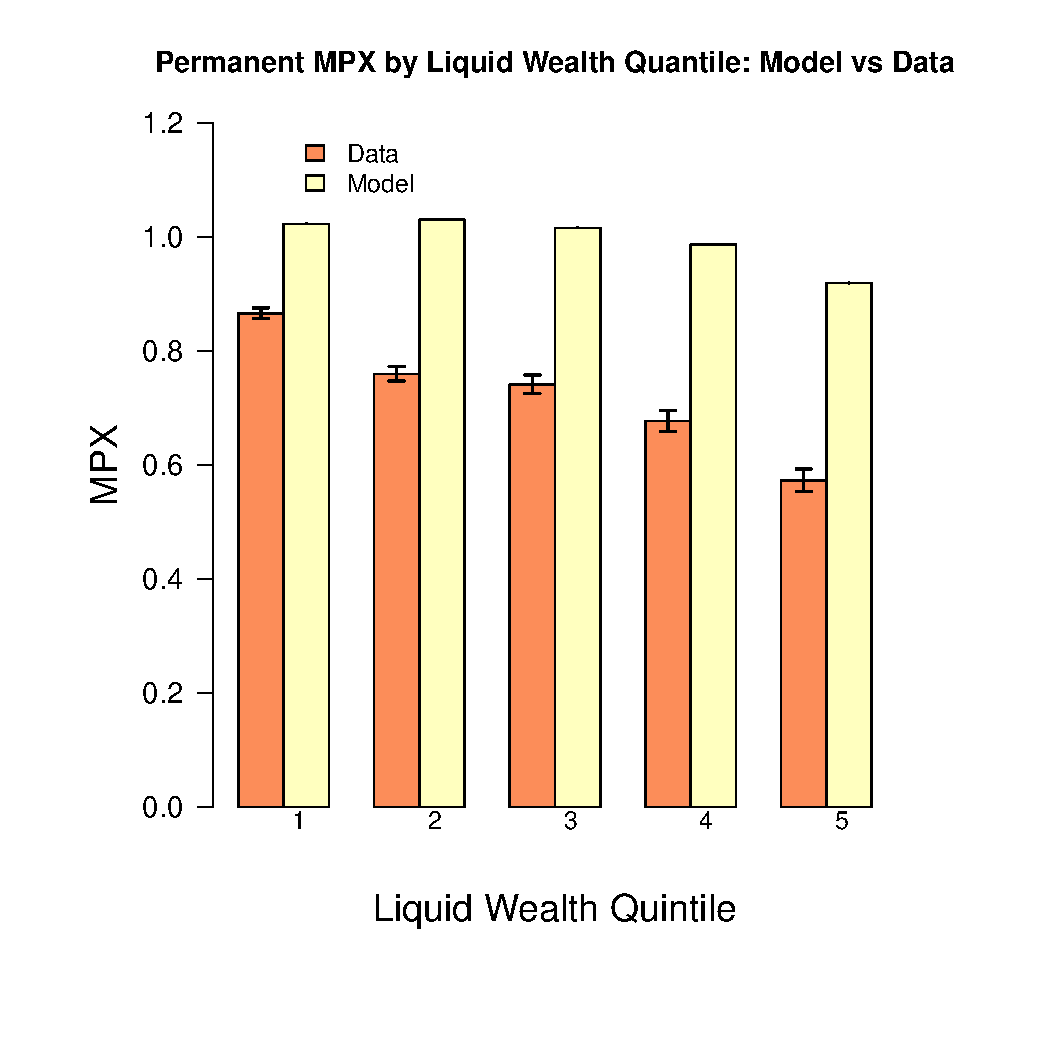
\includegraphics[scale=0.35]{../Figures/CSTW_perm_denmark.pdf}};
	\end{tikzpicture}
	\column{0.5\linewidth}
	\centering
	\begin{tikzpicture}
	\node (img3) {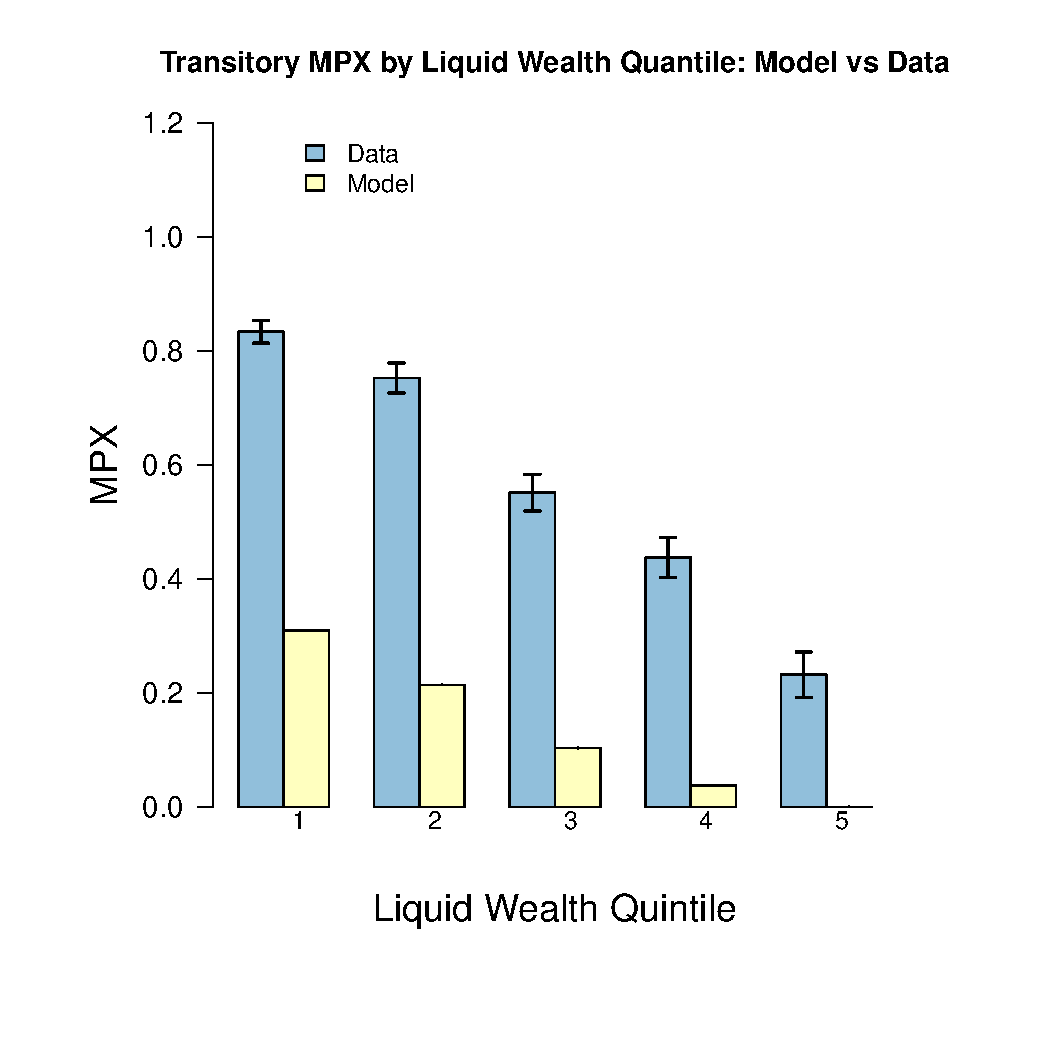
\includegraphics[scale=0.35]{../Figures/CSTW_tran_denmark.pdf}};
	\end{tikzpicture}
\end{columns} 	
}
\frame{
	\frametitle{Preference Shock Model}
	First order problem: Transitory MPCs are too low\\
	\bigskip
	Need to lower $\beta$'s without reducing savings\\
	\bigskip
	Is income risk the only source of precautionary saving?
	\begin{itemize}
		\item In the data, expenditure FAR for volatile than income
		\item Surprise expenses can be large
	\end{itemize}
	Simple extension - add large preference shocks
	\begin{align*}
	\mathbb{E}_t \sum_{i=t}^{\infty} \beta^i \mathcal{X}_i u(\cLevBF_i)
	\end{align*}
}
\end{comment}
\frame
{
	\frametitle{Preference Shock Model: Results}
	\begin{columns}
	\column{0.5\linewidth}
	\centering
	\begin{tikzpicture}
	\node (img1) {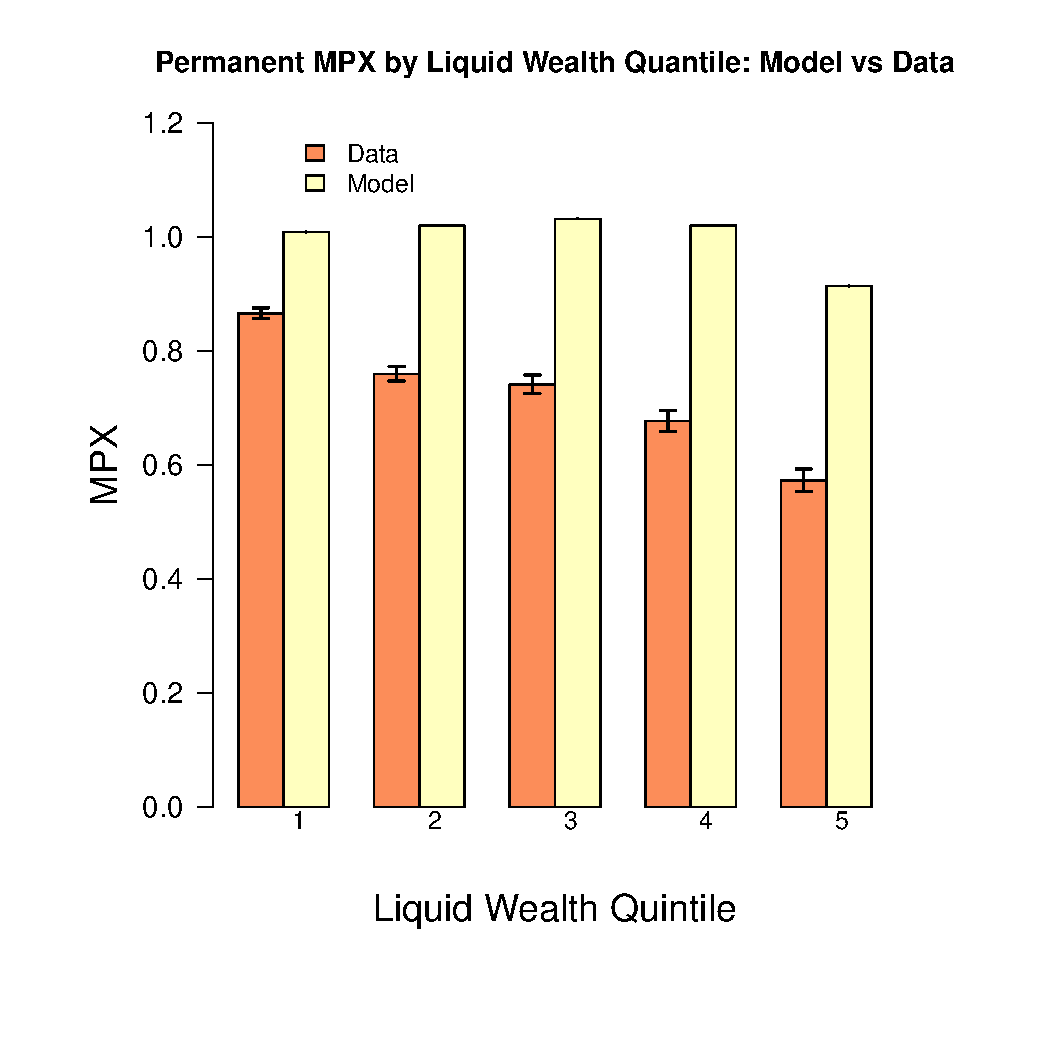
\includegraphics[scale=0.35]{../Figures/CSTW_perm_denmark_pref.pdf}};
	\end{tikzpicture}
	\column{0.5\linewidth}
	\centering
	\begin{tikzpicture}
	\node (img3) {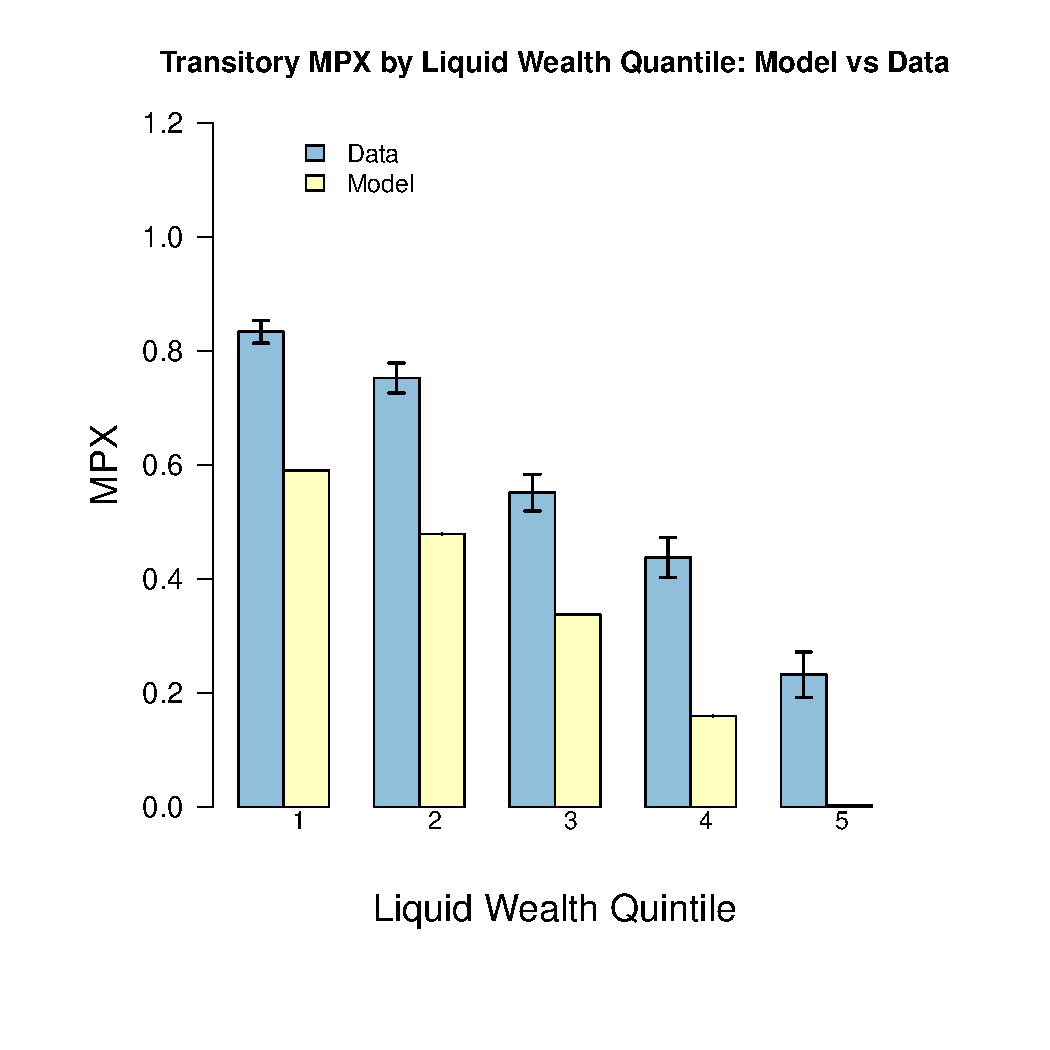
\includegraphics[scale=0.35]{../Figures/CSTW_tran_denmark_pref.pdf}};
	\end{tikzpicture}
\end{columns} 
}
\section{Conclusion}
\frame{
	\frametitle{Conclusion}
	\begin{itemize}
		\item We have designed a new method to estimate consumption responses to income shocks
		\item It appears to work well, both in theory and practice
		\item We can use it to show that heterogeneity plays a key role in monetary policy transmission
	\end{itemize}
	\bigskip
	Thank you!
}
\appendix
\section{MPC vs MPX}
\frame
{
	\frametitle{Durables}
	We have data on value of household cars\\
	\begin{itemize}
		\item Construct expenditure excluding car purchases and sales
		\begin{align*}
		C_T^{\text{nocar}} = C_T - \Delta \text{CarValue}
		\end{align*}
		\item Construct proxy for non durable consumption (Cars $\approx 42.1\%$ durable expenditure)
		\begin{align*}
		C_T^{\text{nondurable}} = C_T - \frac{1}{0.421}\Delta \text{CarValue}
		\end{align*}
	\end{itemize}
}
\frame
{
	\frametitle{Durables}
	\begin{center}
		\begin{tikzpicture}
		\node (img1) {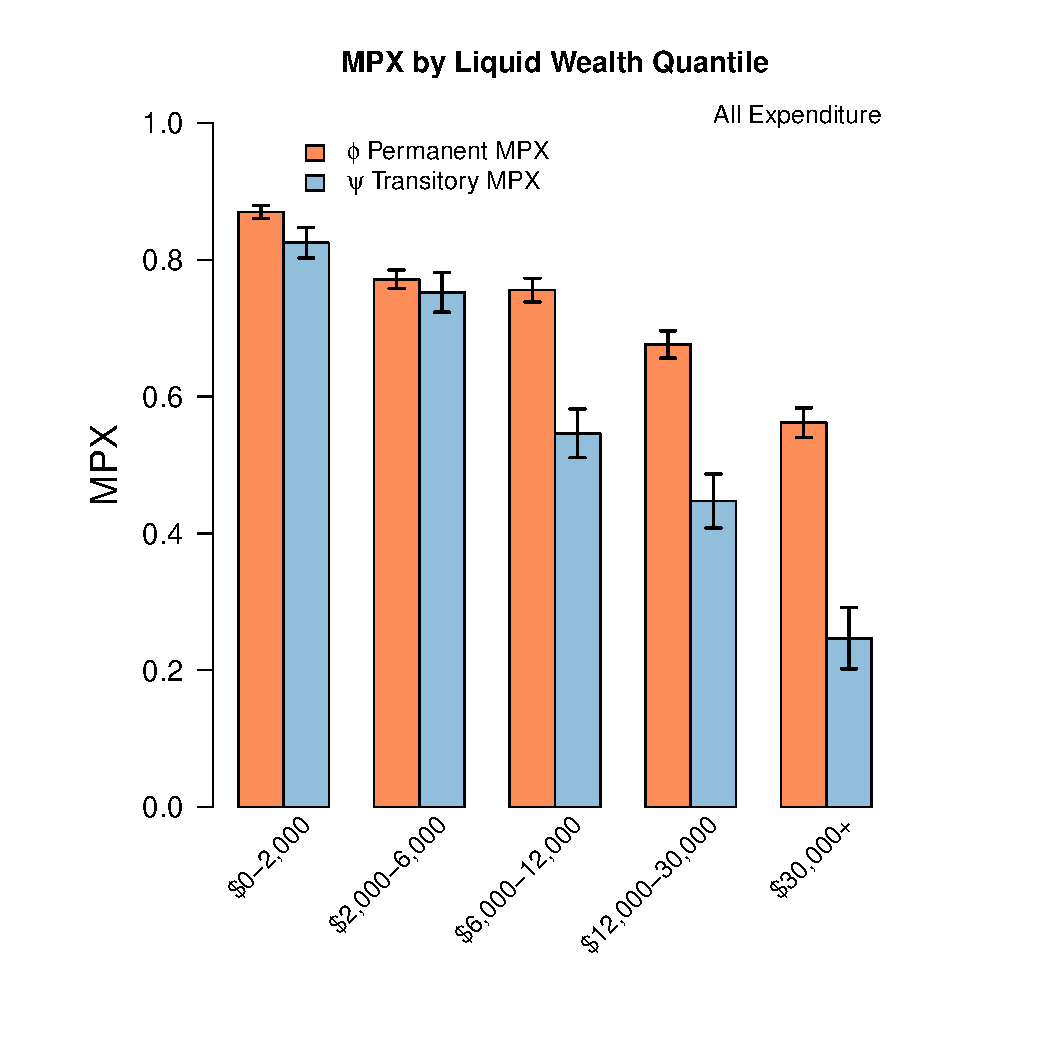
\includegraphics[scale=0.4]{../Figures/MPXByDurables_all.pdf}};
		\pause
		\node (img2)
		{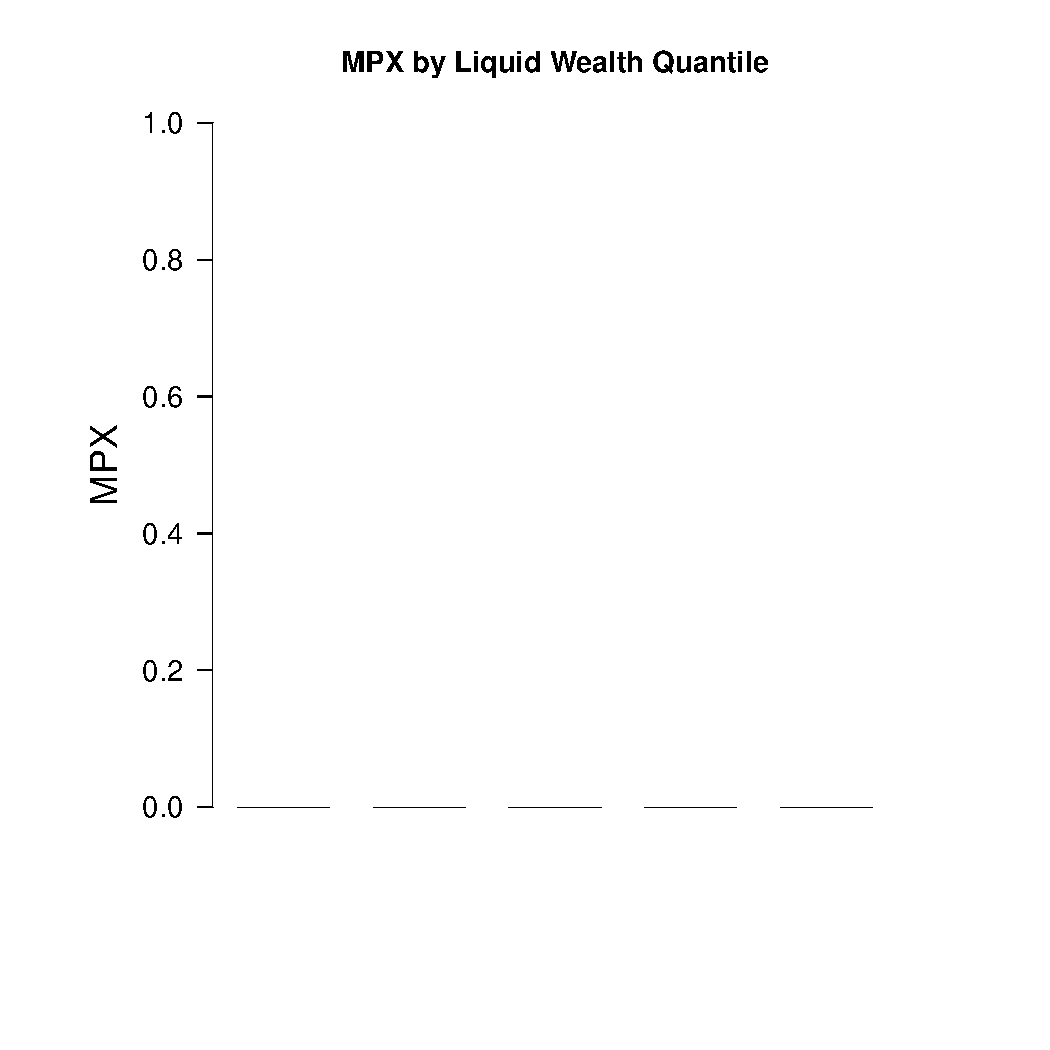
\includegraphics[scale=0.4]{../Figures/MPXByDurables_blank.pdf}};
		\node (img3) {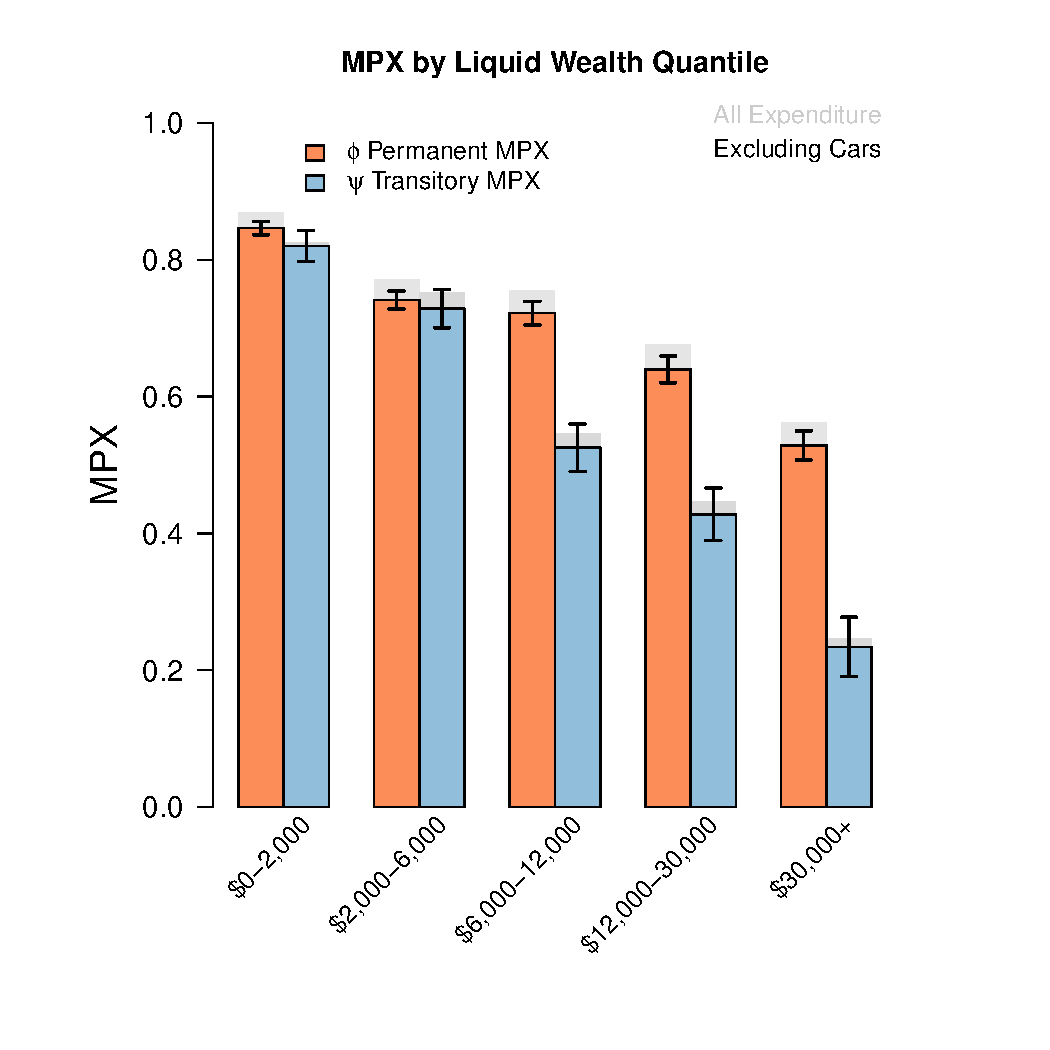
\includegraphics[scale=0.4]{../Figures/MPXByDurables_nocar.pdf}};
		\pause
		\node (img4)
		{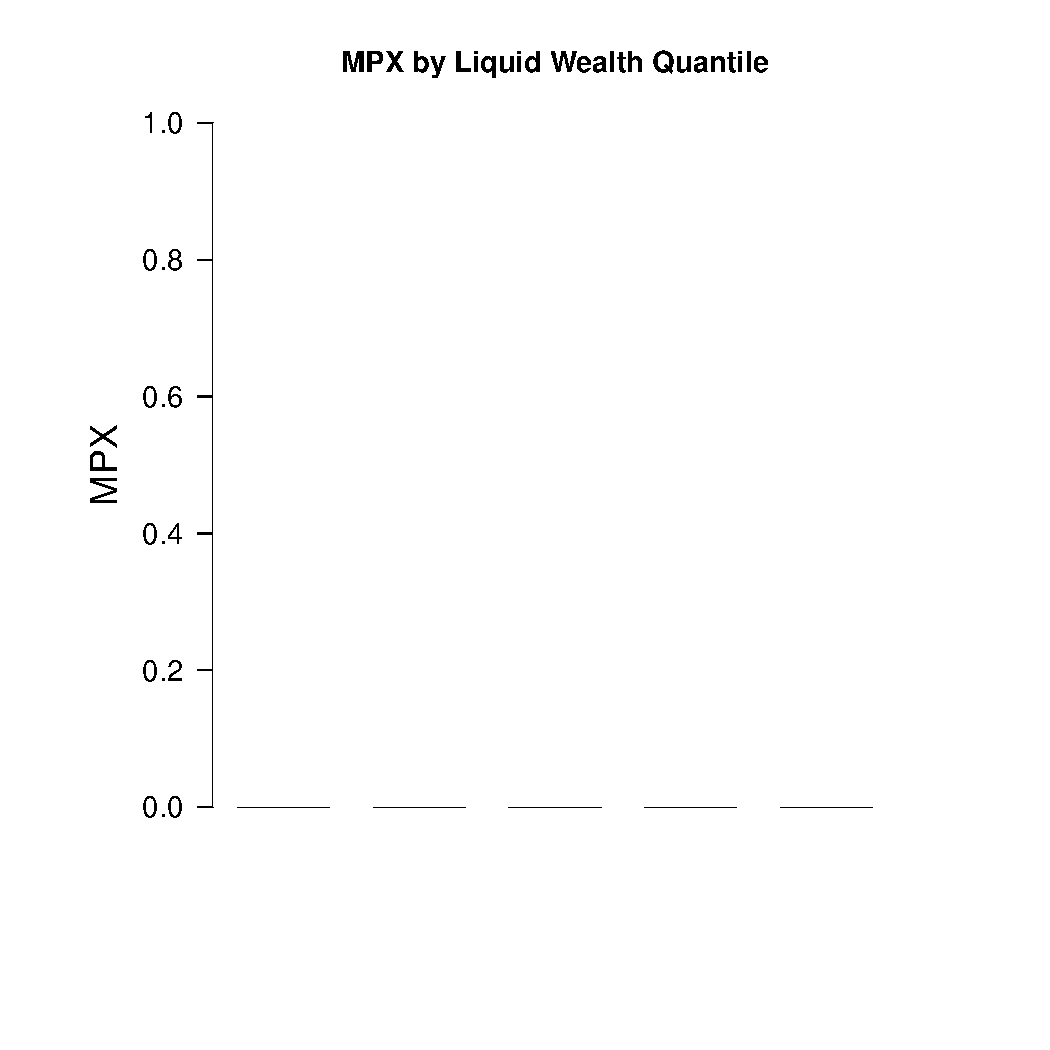
\includegraphics[scale=0.4]{../Figures/MPXByDurables_blank.pdf}};
		\node (img5) {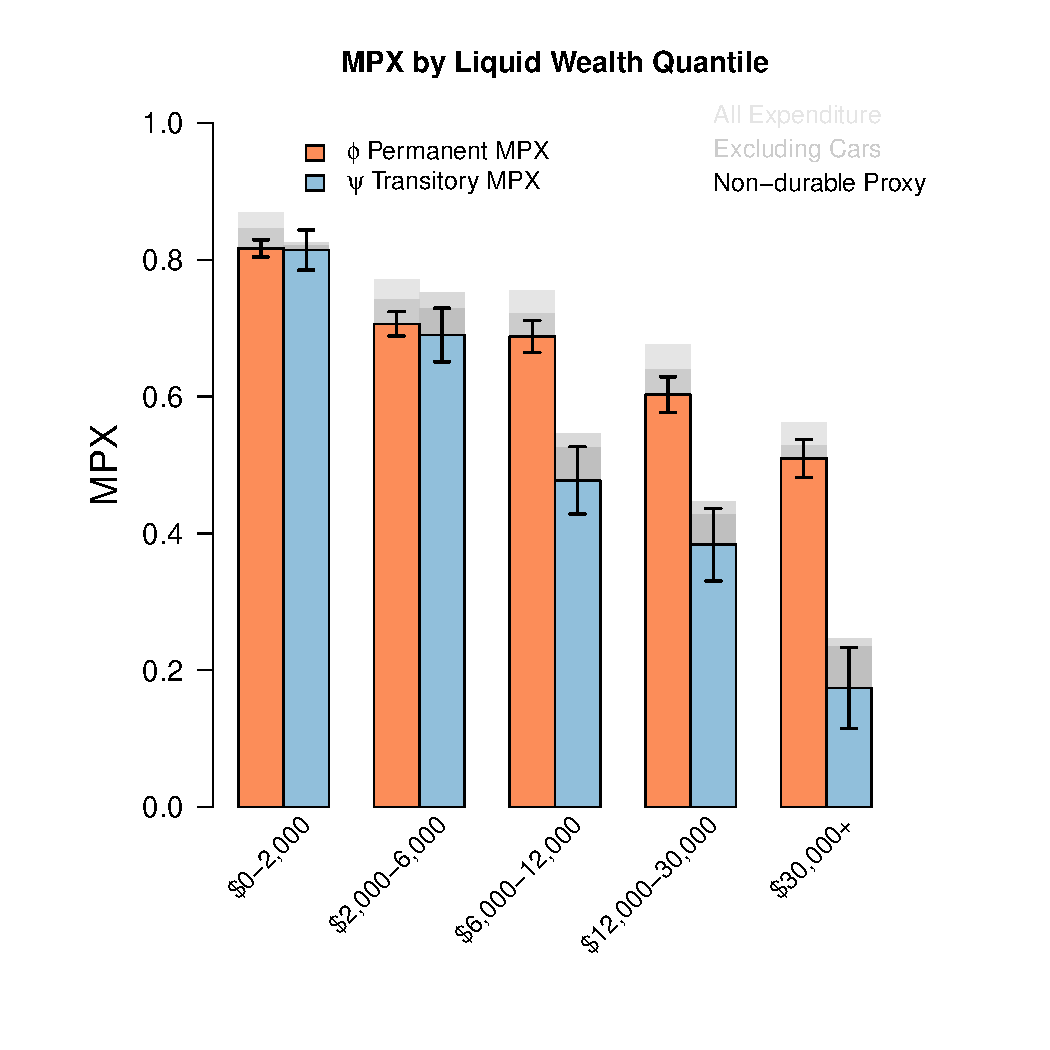
\includegraphics[scale=0.4]{../Figures/MPXByDurables_nodurableproxy.pdf}};
		\onslide<1->
		\end{tikzpicture}
	\end{center}
}
\section{Appendix}
\frame{
	\frametitle{Evidence of Consumption Decay Within 2 Years}
	\label{cons_decay}
	\begin{columns}
	\column{0.35\linewidth}
	\begin{figure}
	From \cite{fagereng_mpc_2016}
	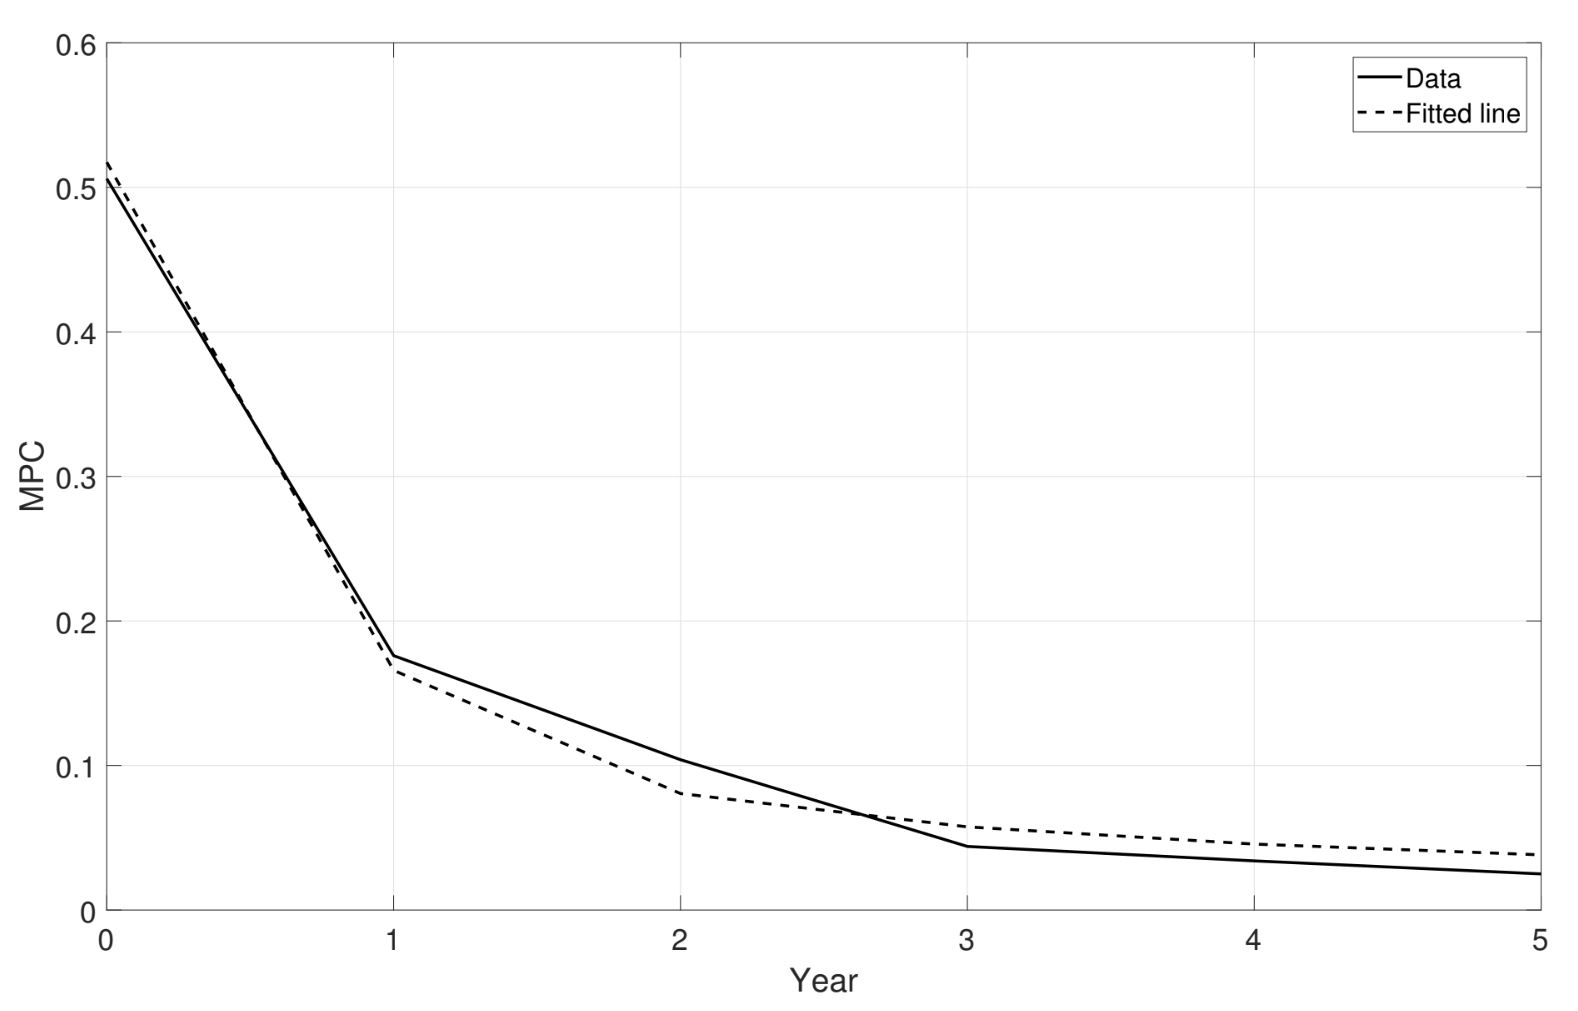
\includegraphics[scale=0.3]{../Figures/norway_cons_decay.JPG}
	\end{figure}
	\column{0.5\linewidth}
	\begin{figure}
	From \cite{gelman_what_2016}
	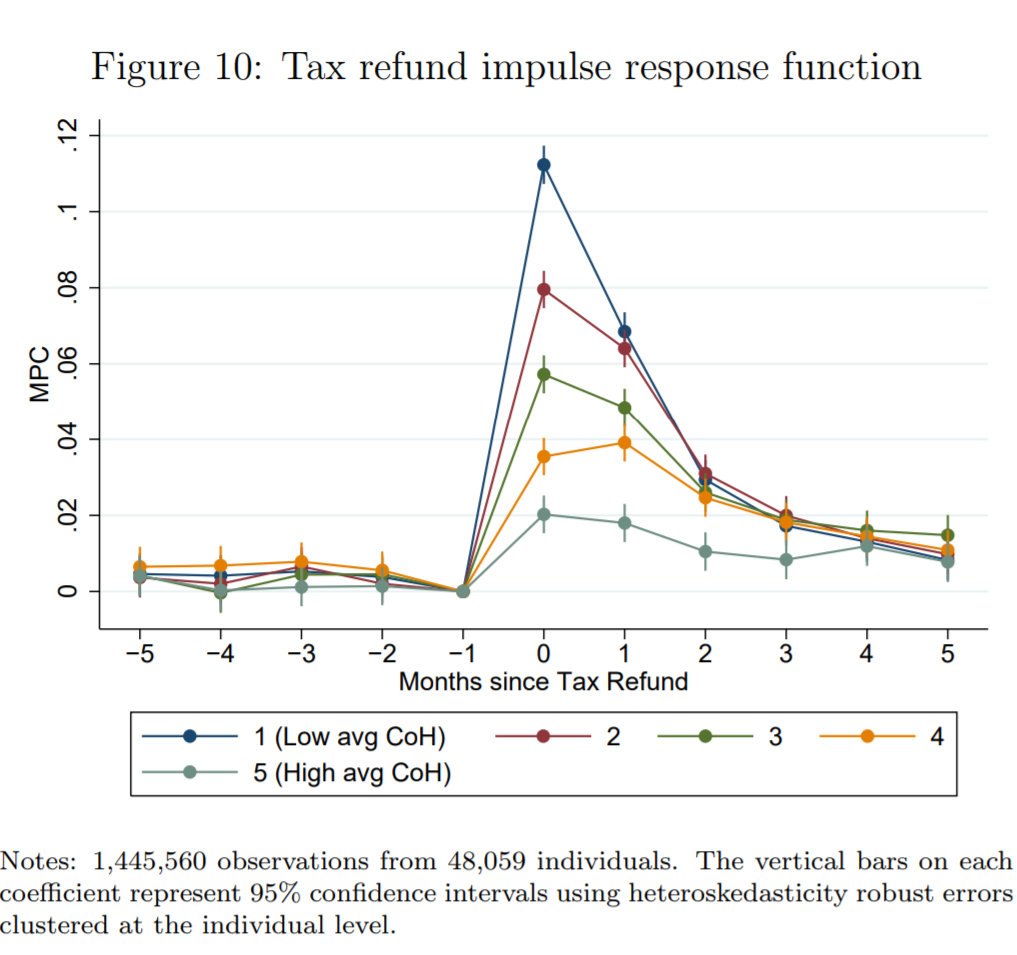
\includegraphics[scale=0.1]{../Figures/gelman_cons_decay.png}
	\end{figure}
	\end{columns}
	\hyperlink{cons_identification}{\beamerbutton{Back}}
}
\frame
{
	\frametitle{MPX by Net Wealth}
	\label{MPXbyNetWealth}
	\begin{columns}
		\column{0.5\linewidth}
		\centering
		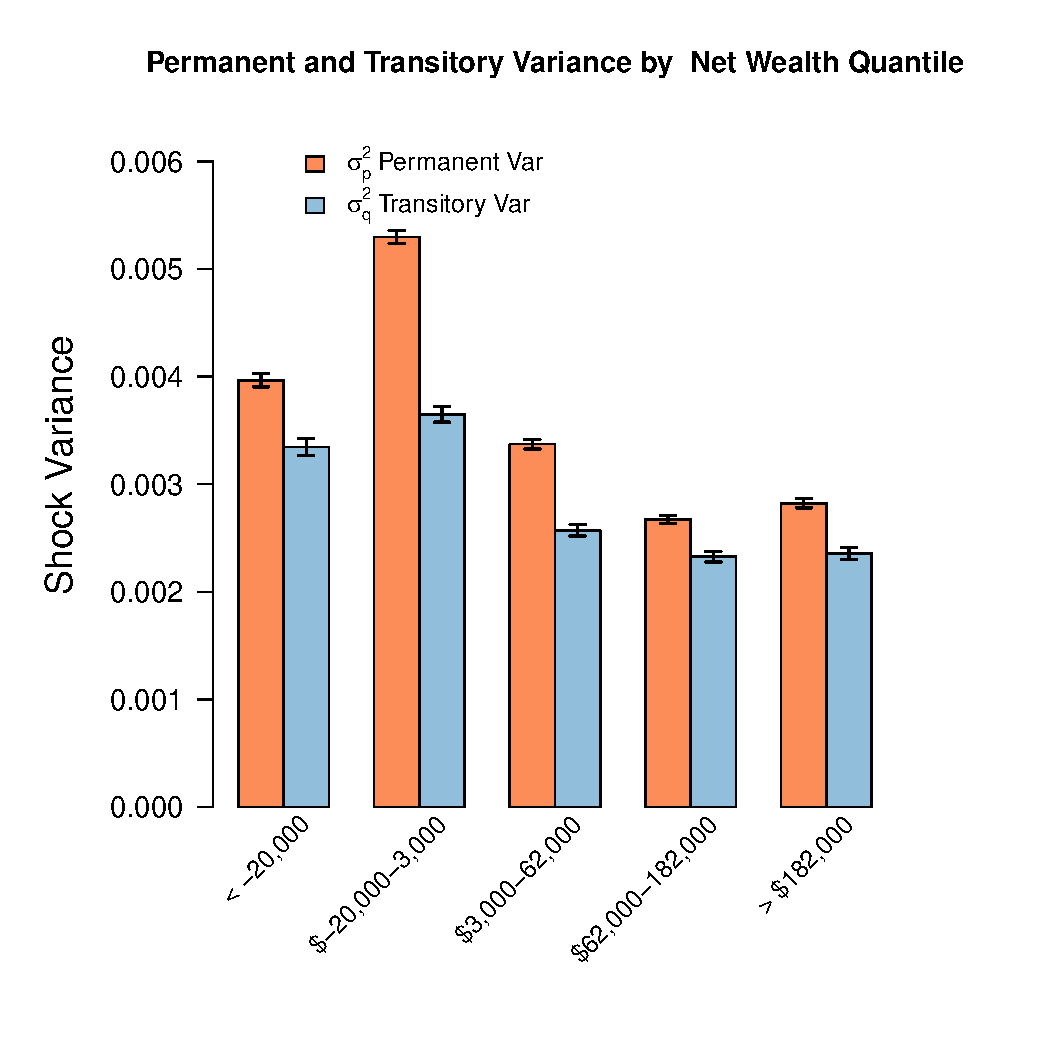
\includegraphics[scale=0.35]{../Figures/VarianceByNetWealth_level_lincome_head.pdf}
		\column{0.5\linewidth}
		\centering
		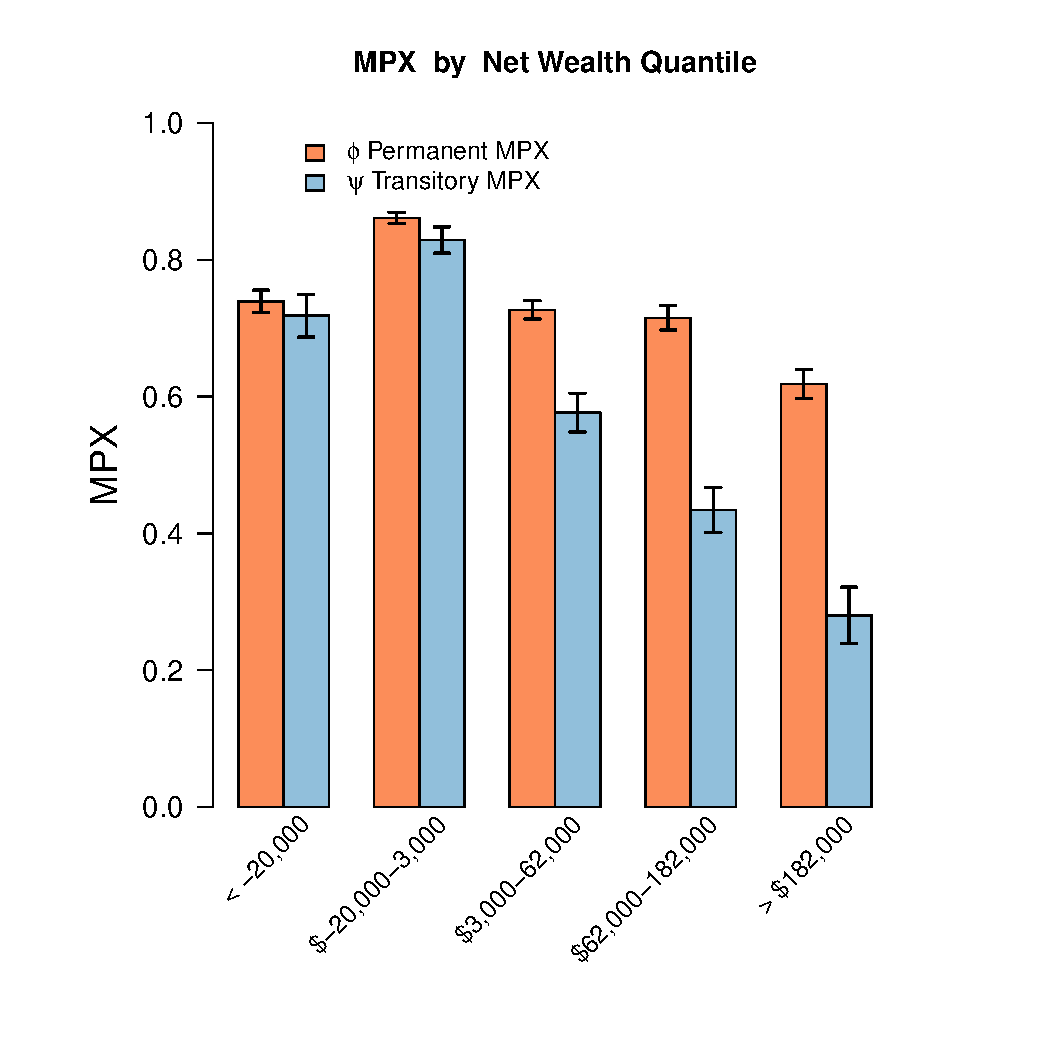
\includegraphics[scale=0.35]{../Figures/MPXByNetWealth_level_lincome_head.pdf}
	\end{columns} 	
	\hyperlink{MPXbyLiquidWealth}{\beamerbutton{Back}}
}
\frame{
	\frametitle{Interest Rate Exposure: Out of Sample}
	\label{OutOfSample}
	\textit{Total} URE sums to zero - this is not true for our household sample \\
	\bigskip
	\tiny
	\input ../Tables/URE_table.tex \\
	\vspace{0.2cm}
	\hyperlink{aggregation}{\beamerbutton{Back}}
}
\frame{
	\frametitle{Summary Statistics}
	\label{summary_stats}
\begin{center} 
	\label{table:SummaryStatistics}
	\input\econtexRoot/Tables/summary_statistics.tex 
\end{center}
	\vspace{0.2cm}
\hyperlink{data_expenditure}{\beamerbutton{Back}}
}

\frame[t]
{
	\frametitle{Aside: Why Not Blundell, Pistaferri and Preston 2008?}
		\label{whynotbpp}
	\textbf{Key to BPP Identification}\\
	\bigskip
	$\Delta y_{t+1}=\Delta p_{t+1}+\Delta \varepsilon_{t+1}$ is a \textit{valid instrument} for $\varepsilon_{t}$\tikz[baseline]{\node(transitory){}}\\
	\only<1->{
		\begin{tikzpicture}[remember picture,overlay]
		\node (transitorya)  at ([shift={(-.2,0.1)}]transitory) {};
		\node (transitoryb)  at ([shift={(0.6,0.6)}]transitorya) {};
		\draw[blue,thick,->] (transitorya)  to [in=225,out=45] (transitoryb) node[anchor=south,text = blue] {Transitory shock year $t$};
		\end{tikzpicture}
	}
	\only<2->{
		\begin{itemize}
			\item Negatively correlated with transitory shocks in year $t$
			\begin{center}
				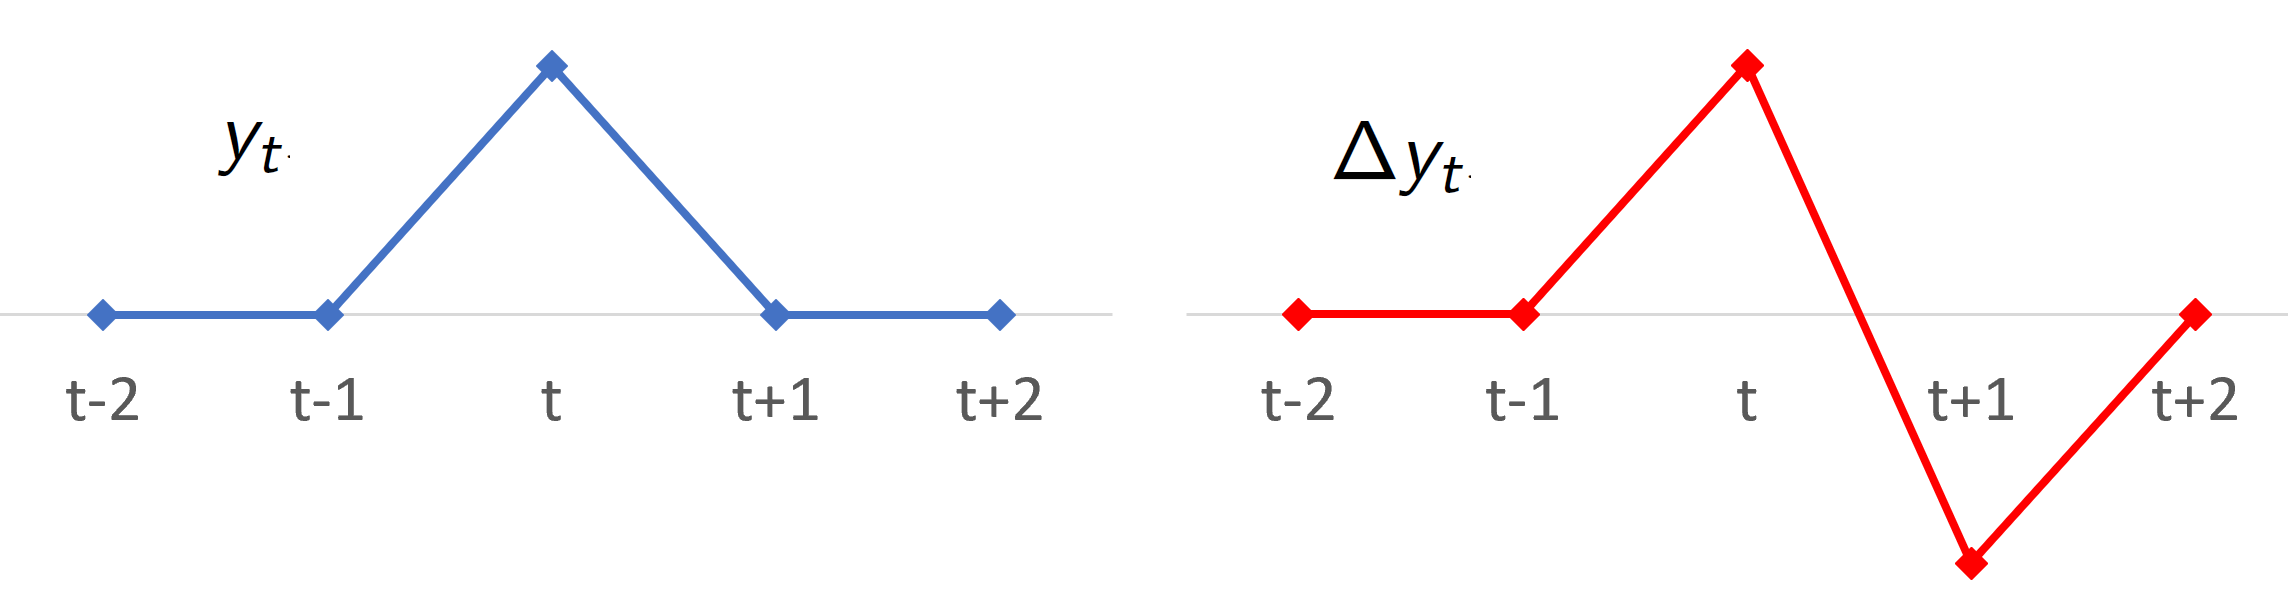
\includegraphics[width=7cm]{./SlideFigures/IncGrowthTran.png}
			\end{center}
		\end{itemize}
	}
	\only<3->{
		\begin{itemize}
			\item U\tikzmark{start}ncorrelated with permanent shocks in year \tikzmark{end}$t$
			\begin{center}
				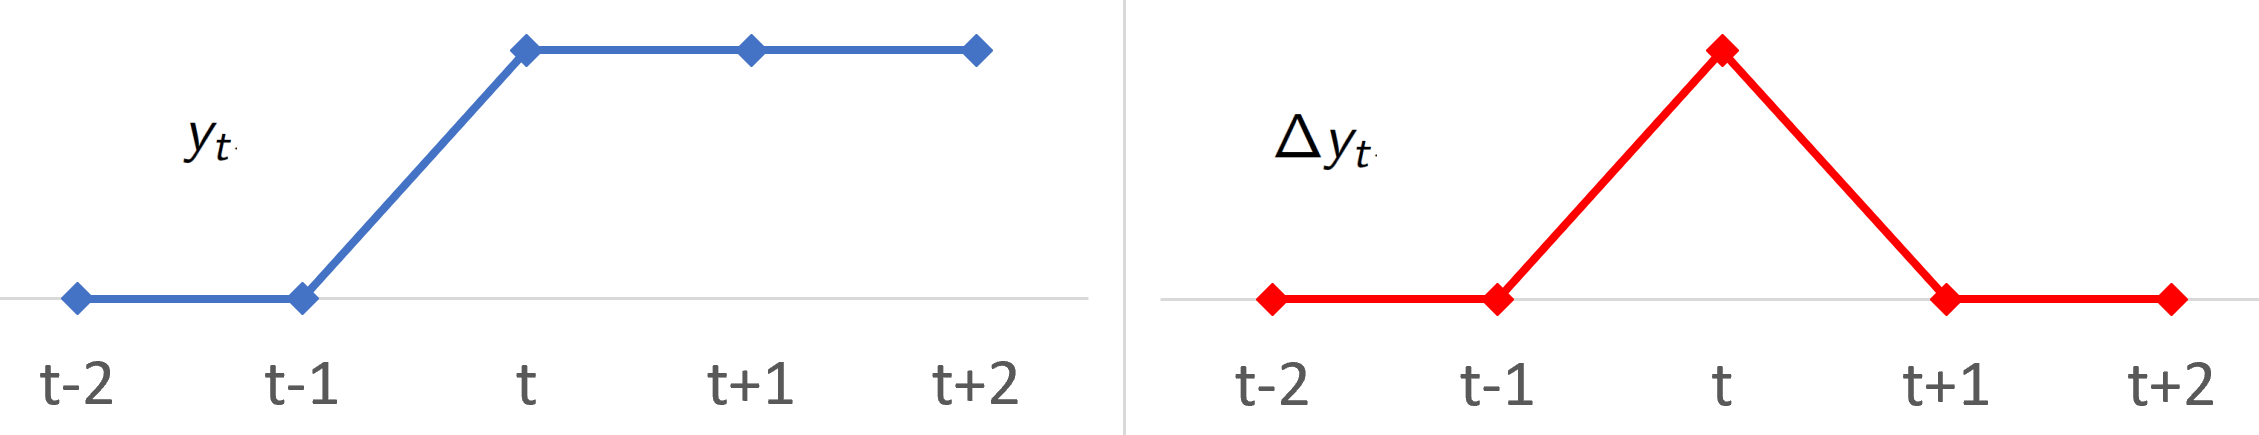
\includegraphics[width=7cm]{./SlideFigures/IncGrowthPerm.png}
			\end{center}
		\end{itemize}
	}
	\only<4->{
		Fails due to the \textbf{Time Aggregation Problem}
		
\begin{tikzpicture}[remember picture,overlay]
		\node[draw,line width=2pt,red,ellipse,inner ysep=10pt,fit={(pic cs:start) (pic cs:end)}] {};
		\end{tikzpicture} 
	}
}
\frame
{
	\frametitle{Aside: Time Aggregation Problem in BPP (Crawley 2018)}
	\begin{columns}
		\column{0.5\linewidth}
		\centering
		\onslide<1->{
			\begin{tikzpicture}
			\node (img1) {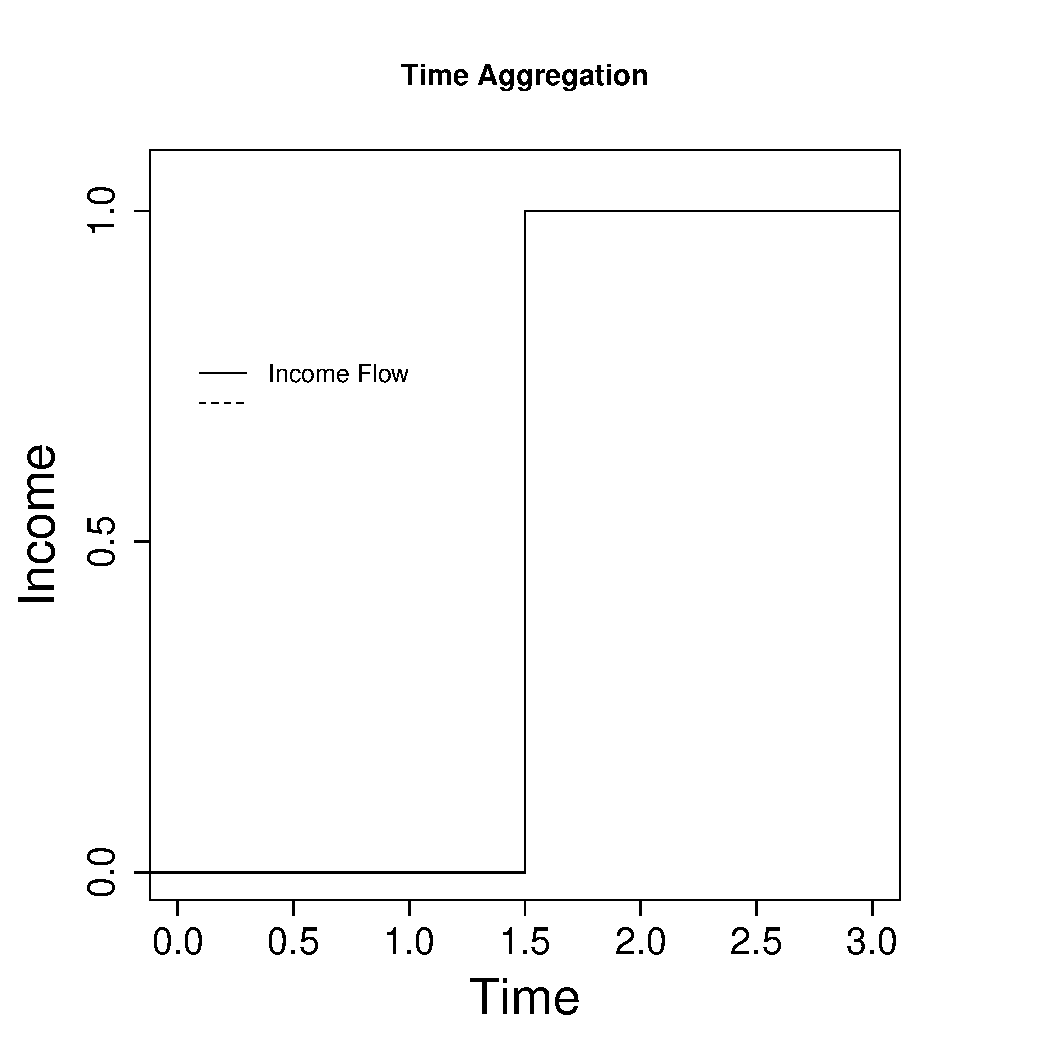
\includegraphics[height=5cm]{../Figures/TimeAggExample1.pdf}};
			\onslide<2->{
				\node (img2) {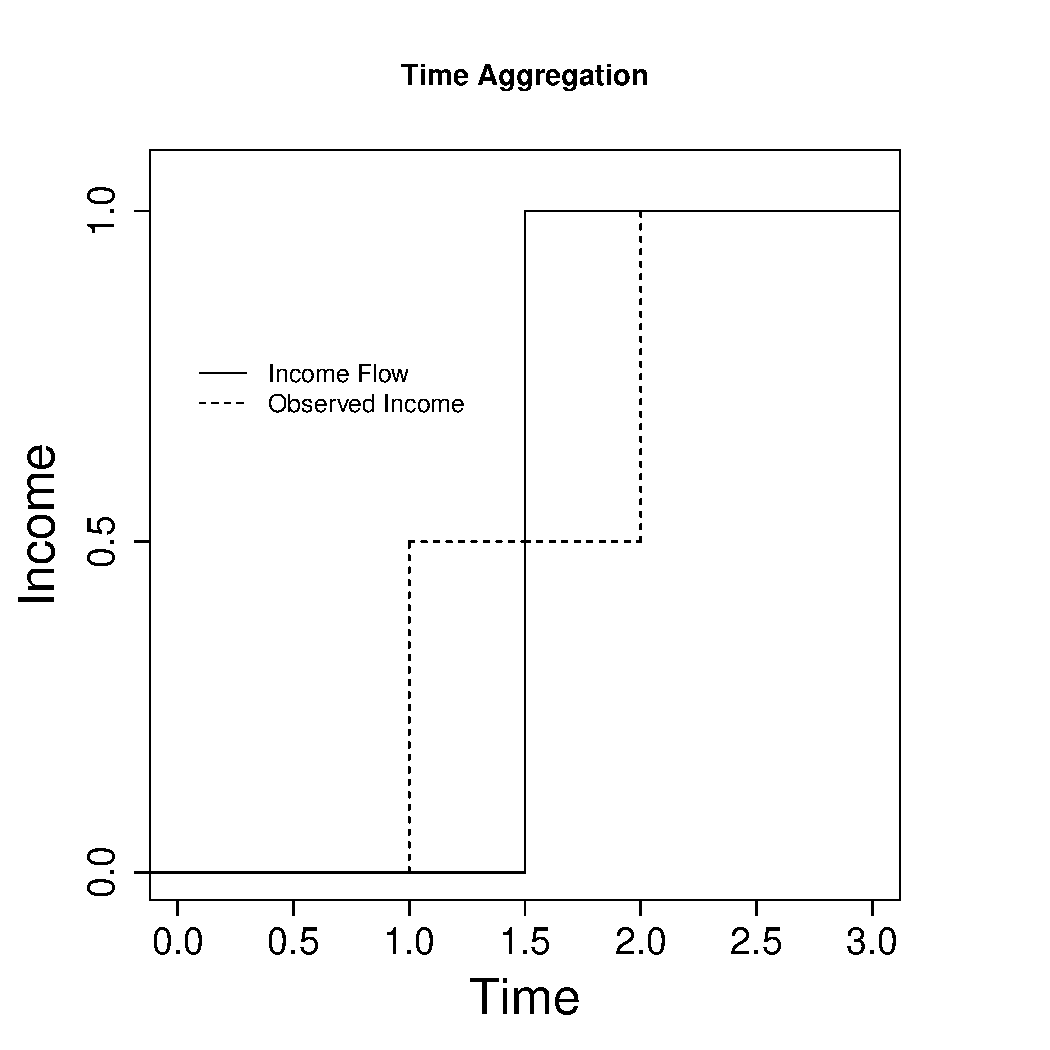
\includegraphics[height=5cm]{../Figures/TimeAggExample2.pdf}};
			}
			\end{tikzpicture}
		}
		\column{0.5\linewidth}
		\onslide<3->{Observed permanent income growth is \textit{positively} autocorrelated\\
			\bigskip
			BPP misinterprets \textit{positive} permanent income shocks as \textit{negative} transitory shocks\\
			\bigskip
			$\implies$ Thinks negative transitory shocks result in consumption \textit{increasing}
		\end{columns}
	}
	\onslide<4->{If the Permanent Income Hypothesis holds, BPP will estimate the MPC to be -0.6}
}
\frame[t]
{
	\frametitle{Data: When is Measurement Error a Problem?}
	\label{measurementerror}
	We have the same issues as the regression:
	\begin{align*}
	\Delta c_i = \alpha + \beta \Delta y_i +\varepsilon_i
	\end{align*}
	That is measurement error in:
	\begin{itemize}
		\item[] $\Delta y_i$ leads to attenuation bias\tikz[baseline]{\node(income){}}
		\item[] $\Delta c_i$ should be uncorrelated with $\Delta y_i$\tikz[baseline]{\node(consumption){}}
	\end{itemize}
	\bigskip
	\only<2>{
	When might this fail?
	\begin{itemize}
		\item Off balance sheet saving
		\item Returns correlated with \textit{changes} in income (e.g. stock compensation)
		\item When insurance is provided by friends and family
	\end{itemize}
	\begin{tikzpicture}[remember picture,overlay]
	\node (incomea)  at ([shift={(0.0,-0.0)}]income) {};
	\node (incomeb)  at ([shift={(0.6,0.6)}]incomea) {};
	\node (consumptiona)  at ([shift={(-4,-0.3)}]consumption) {};
	\node (consumptionb)  at ([shift={(-0.4,-0.4)}]consumptiona) {};
	\draw[blue,thick,->] (incomea)  to [in=225,out=45] (incomeb) node[anchor=west,text = blue] {\begin{tabular}{l} High quality income data  \end{tabular}};
	\draw[blue,thick,->] (consumptiona)  to [in=45,out=45] (consumptionb) node[anchor=north,text = blue] {};
	\end{tikzpicture}
	}
}


\begin{comment}
\section{Model}
\frame
{
	\frametitle{Model}
	How does this compare with a standard buffer-stock saving model?
	\begin{itemize}
		\item Build model to match Danish income process
		\item Allow \textit{heterogeneous discount factors} in order to match the distribution of \textit{liquid} assets in Denmark
		\item See how the distribution of transitory MPX varies with liquid asset holdings
	\end{itemize}
}
\frame
{
	\frametitle{Model}
Given market resources ($\boldmath{\mLevBF}_t$), households in this model maximize expected utility:
\begin{align*}
\mathbb{E}_t \sum_{i=t}^{\infty} \beta^i(1-D)^i  u(\cLevBF_i)
\end{align*}
subject to the constraints:
\begin{align*}
\aLevBF_t = \mLevBF_t - \cLevBF_t \\
\bLevBF_t = R\aLevBF_t \\
\yLevBF_t = \theta_t \pLevBF_t \\
\pLevBF_t = \Psi_t \pLevBF_{t-1} \\
\mLevBF_t = \bLevBF_t + \yLevBF_t
\end{align*}
}
\frame
{
	\frametitle{Calibration}
	\input ../Tables/CalibrationTable.tex
}
\frame
{
	\frametitle{Lorenz Curve}
	Lorenz Curve for Liquid Wealth Holdings
	\centering
	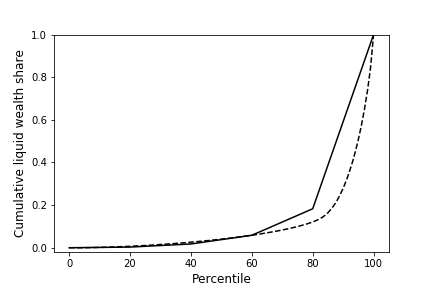
\includegraphics[scale=0.5]{../Figures/Lorenz.png}
}
\frame
{
	\frametitle{Does our Methodology Work?}
	\begin{columns}
	\column{0.5\linewidth}
	\centering
	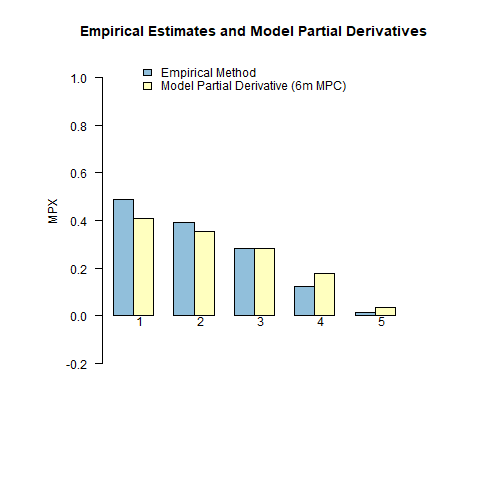
\includegraphics[scale=0.35]{../Figures/MPC_accuracy.png}
	\column{0.5\linewidth}
	\begin{itemize}
		\item Estimate is larger than 6m MPX for low liquid wealth
		\begin{itemize}
		\item Income jumps can be large
		\end{itemize}
		\item Estimate is smaller than 6m MPX for high levels of wealth
		\begin{itemize}
		\item Consumption response lasts more than 2 years
		\end{itemize}
	\end{itemize}
	\end{columns}
}
\frame
{
	\frametitle{Model vs Data}
	How does the model compare with the data?
	\begin{columns}
	\column{0.5\linewidth}
	\centering
	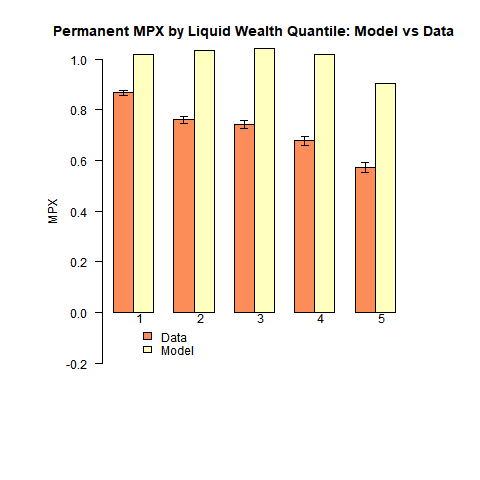
\includegraphics[scale=0.35]{../Figures/CSTW_perm_denmark.png}
	\column{0.5\linewidth}
	\centering
	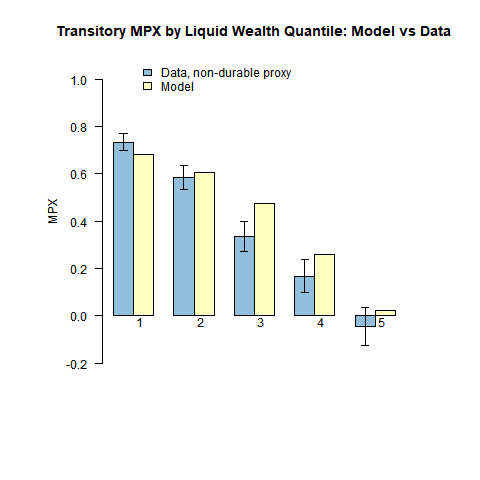
\includegraphics[scale=0.35]{../Figures/CSTW_tran_denmark.png}
	\end{columns} 
}
\section{Threats to Identification}
\frame
{
	\frametitle{Endogenous Income Shocks}
	\begin{itemize}
		\item Household's consumption preference highly variable
		\item Hours worked is endogenous
	\end{itemize}
	The household maximizes:
	\begin{align*}
	\mathbb{E}_t \sum_{n=t}^{\infty} \beta^n \Bigg(\mathcal{X}_n \frac{ \cLevBF_n^{1-\rho}}{1-\rho}-\frac{\lLevBF_n^{1+\frac{1}{\xi}}}{1+\frac{1}{\xi}} \Bigg)
	\end{align*}
	\begin{itemize}
	\item Frisch elasticity $\xi$ 
	\item Preference shock $\mathcal{X}$
	\end{itemize}
}
\frame
{
	\frametitle{Endogenous Income Shocks}
	\input ../Tables/experimental/mpc_laborsupply.tex \\
	\input ../Tables/experimental/psi_laborsupply.tex
}
\frame
{
	\frametitle{Persistent Consumption Response}
	We assume the transitory consumption response lasts less than 2 years \\
	\begin{columns}
	\column{0.5\linewidth}
	\centering 
		High MPC Model\\
	\input ../Tables/experimental/Psi_array1.tex 
	\column{0.5\linewidth}
	\centering
	Low MPC Model\\
	\input ../Tables/experimental/Psi_array2.tex
\end{columns} 
	When MPCs are low, this assumption does not hold in the model, leading to downward bias		
}
\frame
{
	\frametitle{Income Measurement Error}
	Imputation method means measurement error in income shows up in consumption too\\
	Example:
	\begin{itemize}
		\item Actual transitory MPX is zero
		\item 25\% of transitory income variance is due to measurement error
		\item Methodology would result in MPX estimate of 25\%
	\end{itemize}	
	\pause
	But:
	\begin{itemize}
	\item Income is well measured (administrative data)
	\item Bias is much larger for households with small MPCs
	\begin{itemize}
		\item MPX for high liquid wealth households is close to zero
	\end{itemize}
\end{itemize}
}
\frame
{
	\frametitle{Permanent Shocks are AR(1)}
	How does our methodology do if permanent income follows an AR(1) process?
	\begin{align*}
	p_{t} = \rho p_{t-1} + \varepsilon_{t} \\
	y_t = p_t + q_t \\
	c_{t} = \phi y_t + \psi q_t
	\end{align*}
	\centering	
	\input ../Tables/experimental/psi_AR1.tex
}



%%%%%%%%%%%%%%%  bibliography
%%%%%%%%%%%%%%%%%%%%%%%%%%%%%%%%%%%%%%%%%%%%%%%%%%%%%%%%%%%%%%%%%%%%%%%%%%%%%%%%%%%%%%%%%%%%%%%%%%%%%%%%%%%%%%
\tiny

\beamerdefaultoverlayspecification{<*>}
\section{}

\begin{frame}[t,allowframebreaks]
	\frametitle{References}
	
	
	\bibliographystyle{\econtexBibStyle}
	\bibliography{Paper/AllPapers}
\end{frame}

\normalsize
\end{comment}
\bibliographystyle{\econtexBibStyle}
\newsavebox\mytempbib
\savebox\mytempbib{\parbox{\textwidth}{\bibliography{\econtexRoot/AllPapers}}}


\end{document}


